
Im folgenden Kapitel wird die Implementierung auf Basis des zuvor erarbeitet Konzepts als webbasierte Anwendung beschrieben und dokumentiert. Dabei steht vor allem die Architektur der einzelnen Teile, aus denen die Anwendung besteht und die Datenstruktur im Vordergrund.

\subsection{Datenfluss}
Der Datenfluss der Anwendung ist ein typischer Datenfluss für Webapplikationen und in Abbildung \ref{figure:Datenfluss der Anwendung} dargestellt. Die Anwendung besteht aus drei Teilen: Datenbank, Backend und Frontend.

\vspace{20pt}
\begin{center}
    \begin{minipage}{1\linewidth}
        
\includegraphics[width=\linewidth]{Datenfluss}
        \captionof{figure}{Datenfluss der Anwendung}
        \label{figure:Datenfluss der Anwendung}
    \end{minipage}
\end{center}
\vspace{20pt}

Die Datenbank persistiert die Daten der Anwendung. Sie wird durch das Backend verwaltet und gelesen. Das Frontend kann implizit auf diese Daten zugreifen und diese verändern, in dem sie diese vom Backend über eine REST-API anfragt. Das Frontend selbst stellt die Daten in einer benutzerfreundlichen Art und Weise dar und ermöglicht es dem Benutzer die Daten zu verändern, indem es als Benutzeroberfläche für die REST-API des Backends fungiert.

\vspace{20pt}
\begin{center}
    \begin{minipage}{1\linewidth}
        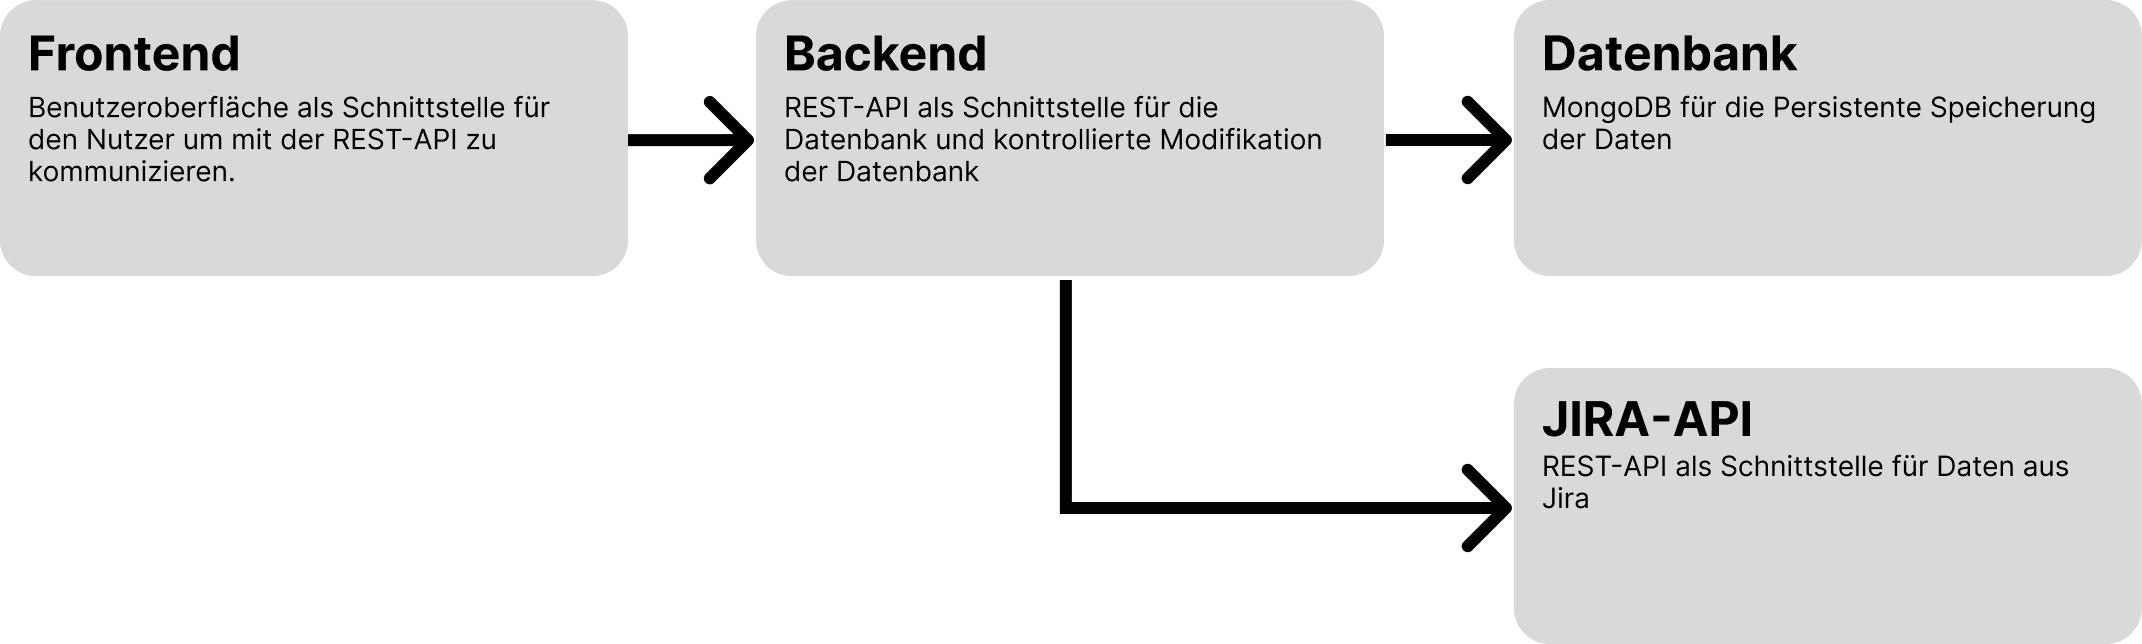
\includegraphics[width=\linewidth]{Datenfluss(inkl Jira)}
        \captionof{figure}{Datenfluss der Anwendung inkl. Jira}
    \end{minipage}
\end{center}
\vspace{20pt}

Hinterlegt der Nutzer ein Jira-Token kommt eine vierte Komponente hinzu. Diese Komponente ist die Jira-API, welche die Daten aus Jira zur Verfügung stellt. Um damit den Datenfluss einheitlich zu gestalten, wird die JIRA-API durch das Backend angesprochen, als wäre es eine Datenbankabfrage. Somit hat das Frontend nur eine einzige Quelle an Information.

\subsection{Datenstruktur}
Die Datenstruktur der Anwendung besteht grundsätzlich aus drei abstrakten und fünf konkreten Klassen. Abstrakten Klassen sind: Entitäten, organisationsbasierende Entitäten und verlinkbare Entitäten. Absolute Klassen sind: Nutzer, Organisation, Level, Gruppe und Aufgabe.

\vspace{20pt}
\begin{center}
    \begin{minipage}{0.8\linewidth}
        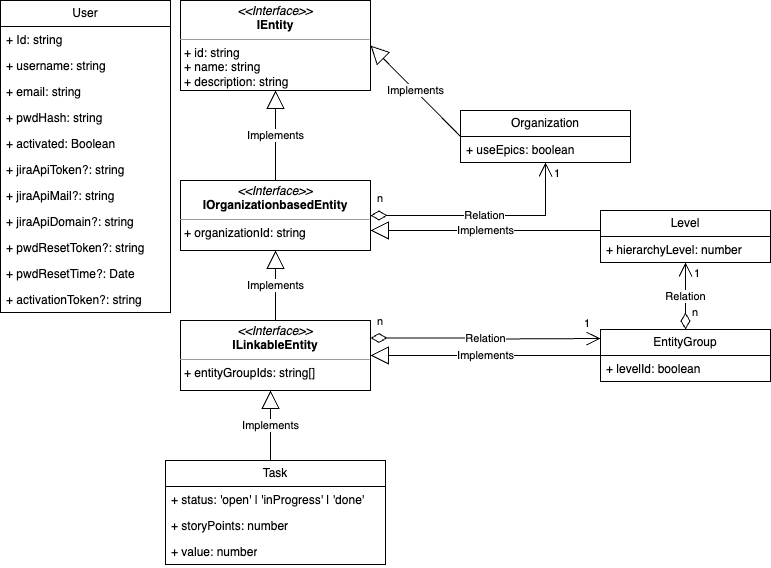
\includegraphics[width=\linewidth]{classDiagramm}
        \captionof{figure}{UML-Diagramm der Datenstruktur}
    \end{minipage}
\end{center}
\vspace{20pt}

Jede absolute Klasse, außer die Nutzer, erben von einer oder mehreren abstrakten Klassen. Entitäten sind allgemeine Objekte innerhalb der Anwendung und stellen die Grundlage der in der Datenbank gespeicherten Datenobjekte dar. Alle Klassen außer Nutzer sind solche Entitäten und implementieren das Interface \verb|IEntity|, welches eine ID zur eindeutigen Identifikation, einen Namen und eine Beschreibung für die Darstellung für den Nutzer beinhaltet. Organisationen und Levels sind direkte Erben dieser Klasse. Die nächste Abstraktionsstufe sind die organisationsbasierenden Entitäten. Diese implementieren zu dem \verb|IEntity| Interface noch \verb|IOrganizationBasedEntity|, welches die ID einer Organisation voraussetzt und die Entität direkt von einer Organisation abhängig macht. Die letzte Abstraktionsstufe sind die verlinkbaren Entitäten. Diese implementieren zu dem \verb|IOrganizationBasedEntity| Interface noch \verb|ILinkableEntity|, welches eine Liste von IDs voraussetzt, mit dem gespeichert wird, mit welchen anderen verlinkbaren Entitäten das Objekt verlinkt ist. Aufgaben und Gruppen sind solche verlinkbare Entitäten.

\subsection{Backend-Architektur}
Das Backend ist eine REST-API, geschrieben mit Node.js und Express in TypeScript und verwendet mongoose als Datenbank-API für MongoDB. Die Architektur beschreibt den Datenfluss mit drei allgemeinen Komponenten: Router, Controller und Service.
Der Router bestimmt für einen Request welche Funktion eines Controllers aufgerufen wird. Die aufgerufene Controller-Funktion beinhaltet die Business-Logik, die an den Request gebunden ist und führt diese aus. Um Daten aus der Datenbank zu holen oder die geholten Daten zu modifizieren gibt es für jede Datenklasse einen Service, der die benötigten Datenbankoperationen implementiert und somit von der Business-Logik trennt. Für die Interaktion mit der Datenbank muss außerdem ein sogenanntes Model definiert werden, welches die Beschreibung der Klasse also der Type in TypeScript mit der Datenbank-Collection und den Objekten darin verknüpft.

\vspace{20pt}
\begin{center}
    \begin{minipage}{1\linewidth}
        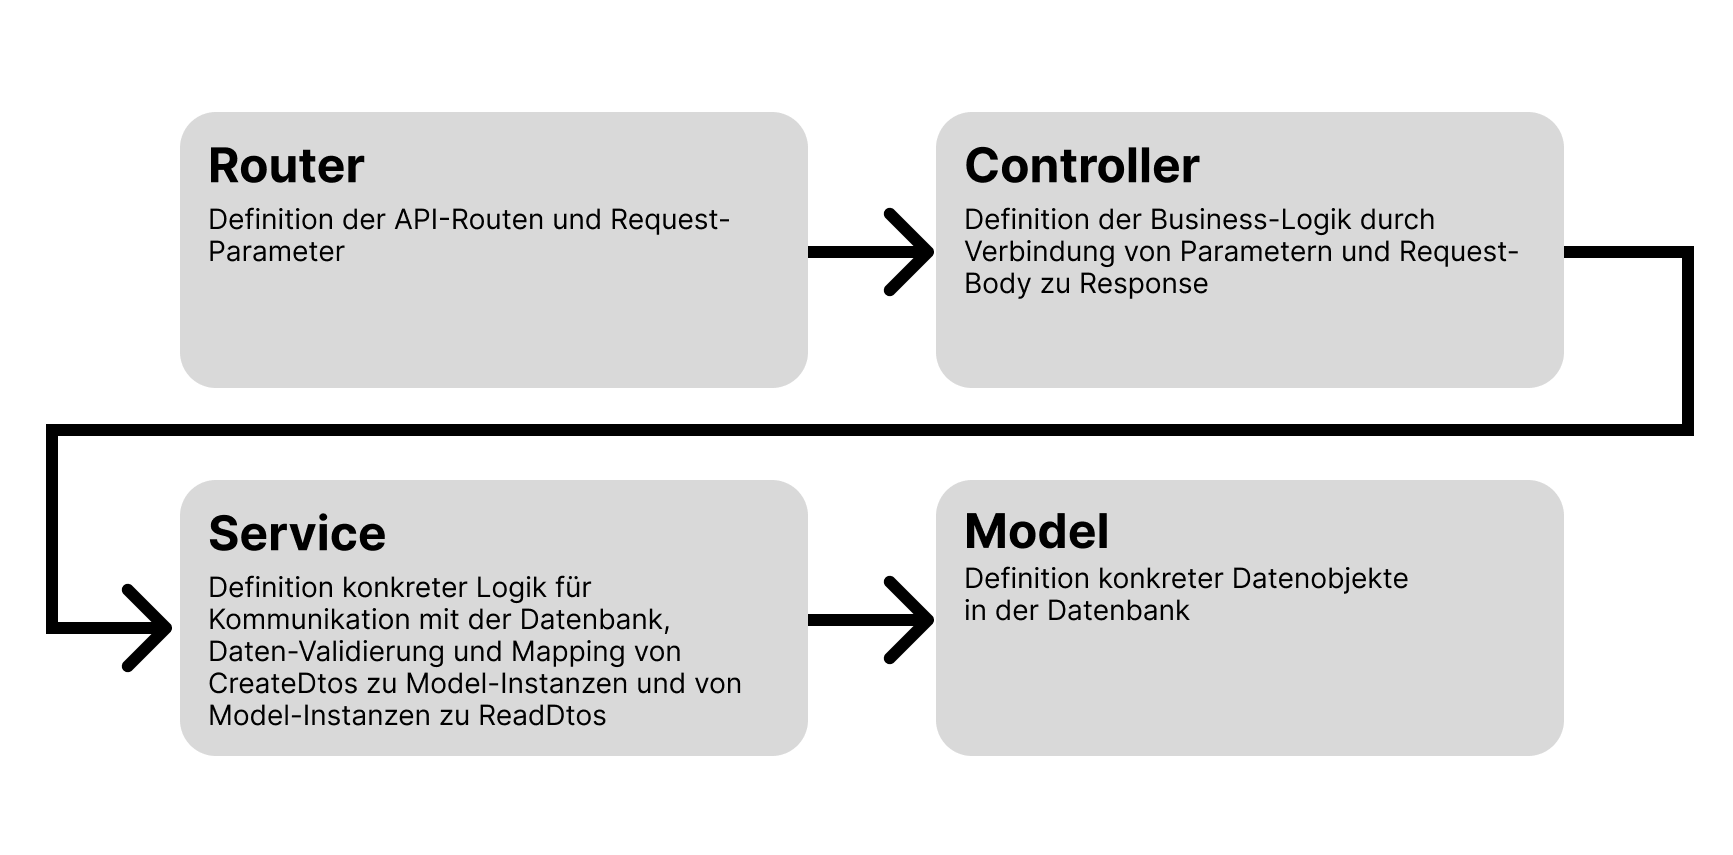
\includegraphics[width=\linewidth]{BE-Struktur}
        \captionof{figure}{Backend Architektur}
    \end{minipage}
\end{center}
\vspace{20pt}

Für die konkrete Kommunikation mit der REST-API werden zu den konkreten Datenobjekten innerhalb der Datenbank zwei weitere Klassen je Objekt-Klasse definiert. Diese Klassen sind sogenannte Data transfer Objects (DTO). DTOs dienen dazu die Kommunikation zu generalisieren und definieren die Daten, die der Konsument der API durch einen Request erhalten kann und die Daten, die ein Konsument der API zur Verfügung stellen kann, um z. B. ein neues Objekt in der Datenbank zu erstellen. Die zusätzlichen Klassendefinitionen werden durch diese zwei Anwendungsfälle in Read- und Create-/Update-DTOs unterteilt. Wie Create-/Update-DTOs zu einem internen Model gemappt werden und wie aus einem internen Model ein Read-Dto gemappt wird, definiert ebenfalls der zum Model zugehörige Service.

Der Aufbau des Backends gleicht dem Aufbau der Klassen-Abstraktion. Es gibt für jede abstrakte Klasse eine Struktur welche jeweils eine abstrakte Implementierung für Router, Controller, Services und Model beinhalten.
Zudem gibt es fünf absolute Strukturen für jede der fünf absoluten Klassen, welche von den verschiedenen abstrakten Strukturen erben.

\vspace{20pt}
\begin{center}
    \begin{minipage}{0.7\linewidth}
        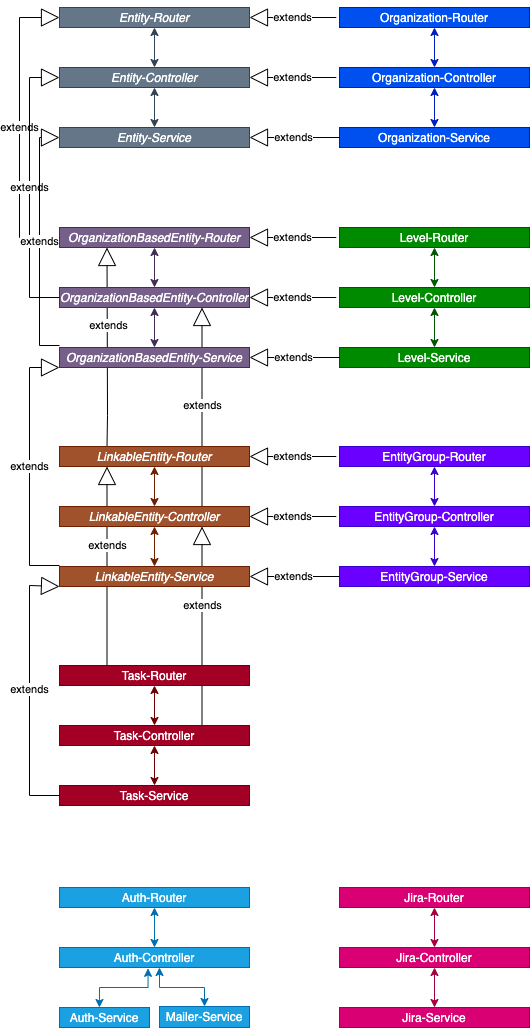
\includegraphics[width=\linewidth]{BackendStruktur}
        \captionof{figure}{Abbildung der BE-Struktur}
    \end{minipage}
\end{center}
\vspace{20pt}

Eine vollständige Dokumentation der API nach Open-API-Spezifikation-3.0.0 im Swagger-Format ist \href{https://bachelor.oedinger.io/api-docs/}{https://bachelor.oedinger.io/api-docs/} verfügbar. Dort sind die für den Client zugänglichen Routen inklusive der benötigten Parameter und den zurückgegebenen Daten dokumentiert.

\vspace{20pt}
\begin{center}
    \begin{minipage}{0.95\linewidth}
        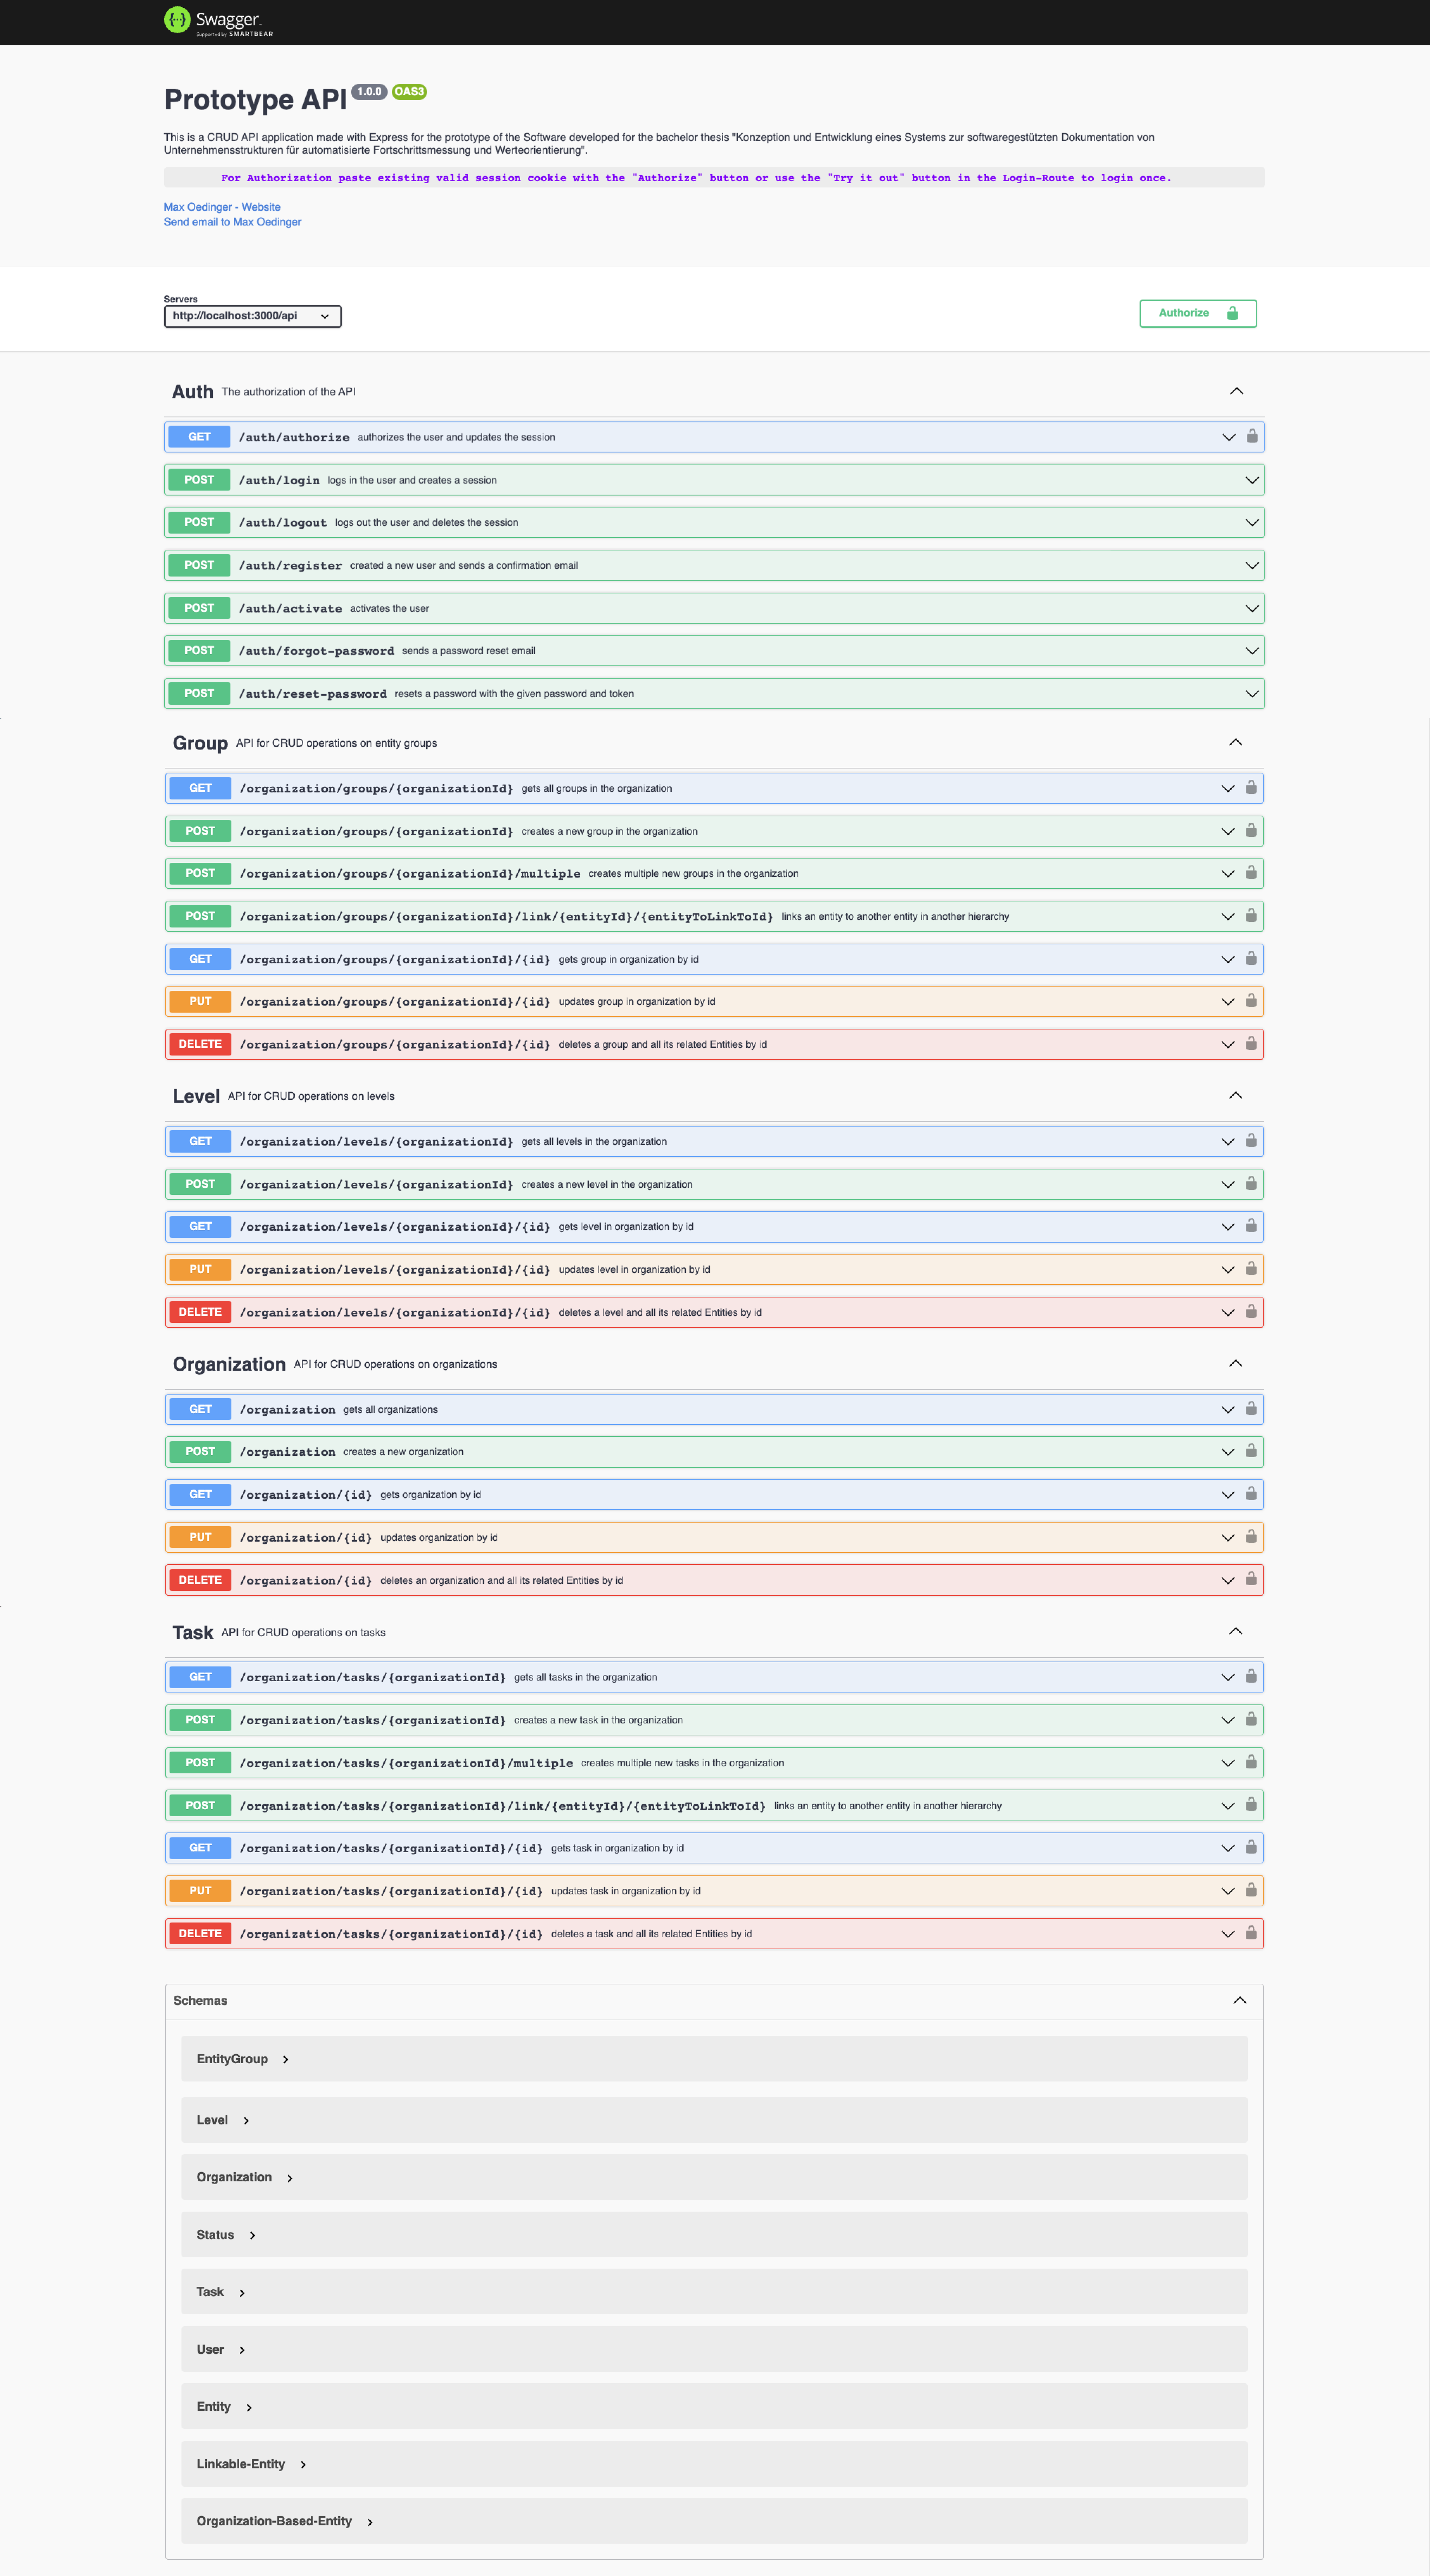
\includegraphics[width=\linewidth]{swagger}
        \captionof{figure}{API-Dokumentation}
    \end{minipage}
\end{center}
\vspace{20pt}

Für die Authentifizierung werden die Node-Packages \verb|express-sessions| und \verb|passport| verwendet. Zusammen mit einer Persistierung in der Datenbank wird hiermit eine Session-Authentifizierung implementiert, die mit Authentication-Cookies funktioniert.

\subsection{Benutzeroberfläche}
Zur initialen Planung wurde zunächst der UX-Entwurf verwendet, um die grobe Struktur der Benutzeroberfläche zu entwickeln. Durch die spezifische Entwicklung verschiedener Features sind immer wieder Lücken im Entwurf aufgefallen und wurden durch weitere UI-Elemente erweitert, um Funktionalitäten abzudecken, die zuvor nicht innerhalb des Prototyps bedacht wurden. Bis zum fertigen Prototyp haben sich viele der konkreten UI-Elemente verändert, allerdings blieb die Seitenstruktur, also welche Informationen auf welcher Seite dargestellt wurden, identisch.

Für die Implementierung wurde als Frontend-/UI-Framework Vue.js verwendet. Vue.js ist eine Framework für die Entwicklung von Single-Page-Webanwendungen. Es ist ein JavaScript-Framework, welches auf dem Model-View-ViewModel (MVVM) basiert. Die UI wurde also in verschiedene Komponenten zerteilt. Die Komponenten werden in zwei Kategorien unterteilt: Views und Components. Views sind logisch voneinander getrennte Seiten der Anwendung, während Components kleinere Bestandteile der Views zur Vereinfachung der in der View benötigten Logik oder wiederverwendbare UI-Elemente sind. Zur weiteren Strukturierung werden hier noch sogenannte Layouts verwendet. Layouts stellen die Grundstruktur der Anwendung dar, welche von mehreren Views verwendet wird. Für das Styling der Anwendung wurde das CSS-Framework Tailwind-CSS verwendet. Dabei handelt es sich aber um kein Design-Framework, sondern lediglich um eine alternative Art natives CSS zu verwenden. Dementsprechend hat das Frontend sein eigenes Design, welches sich an keine festen Design-Vorgaben eines anderen Systems hält.

\subsubsection{Layouts}
Die Anwendung teilt sich zunächst in zwei solcher Layouts: Authentifizierung und eigentliche Anwendung.

Das Layout der Authentifizierung beschreibt nur die Positionierung der relevanten Elemente in der Mitte des Bildschirms, da sich alle Seiten der Authentifizierung diese Eigenschaft teilen.

\vspace{20pt}
\begin{center}
    \begin{minipage}{0.8\linewidth}
        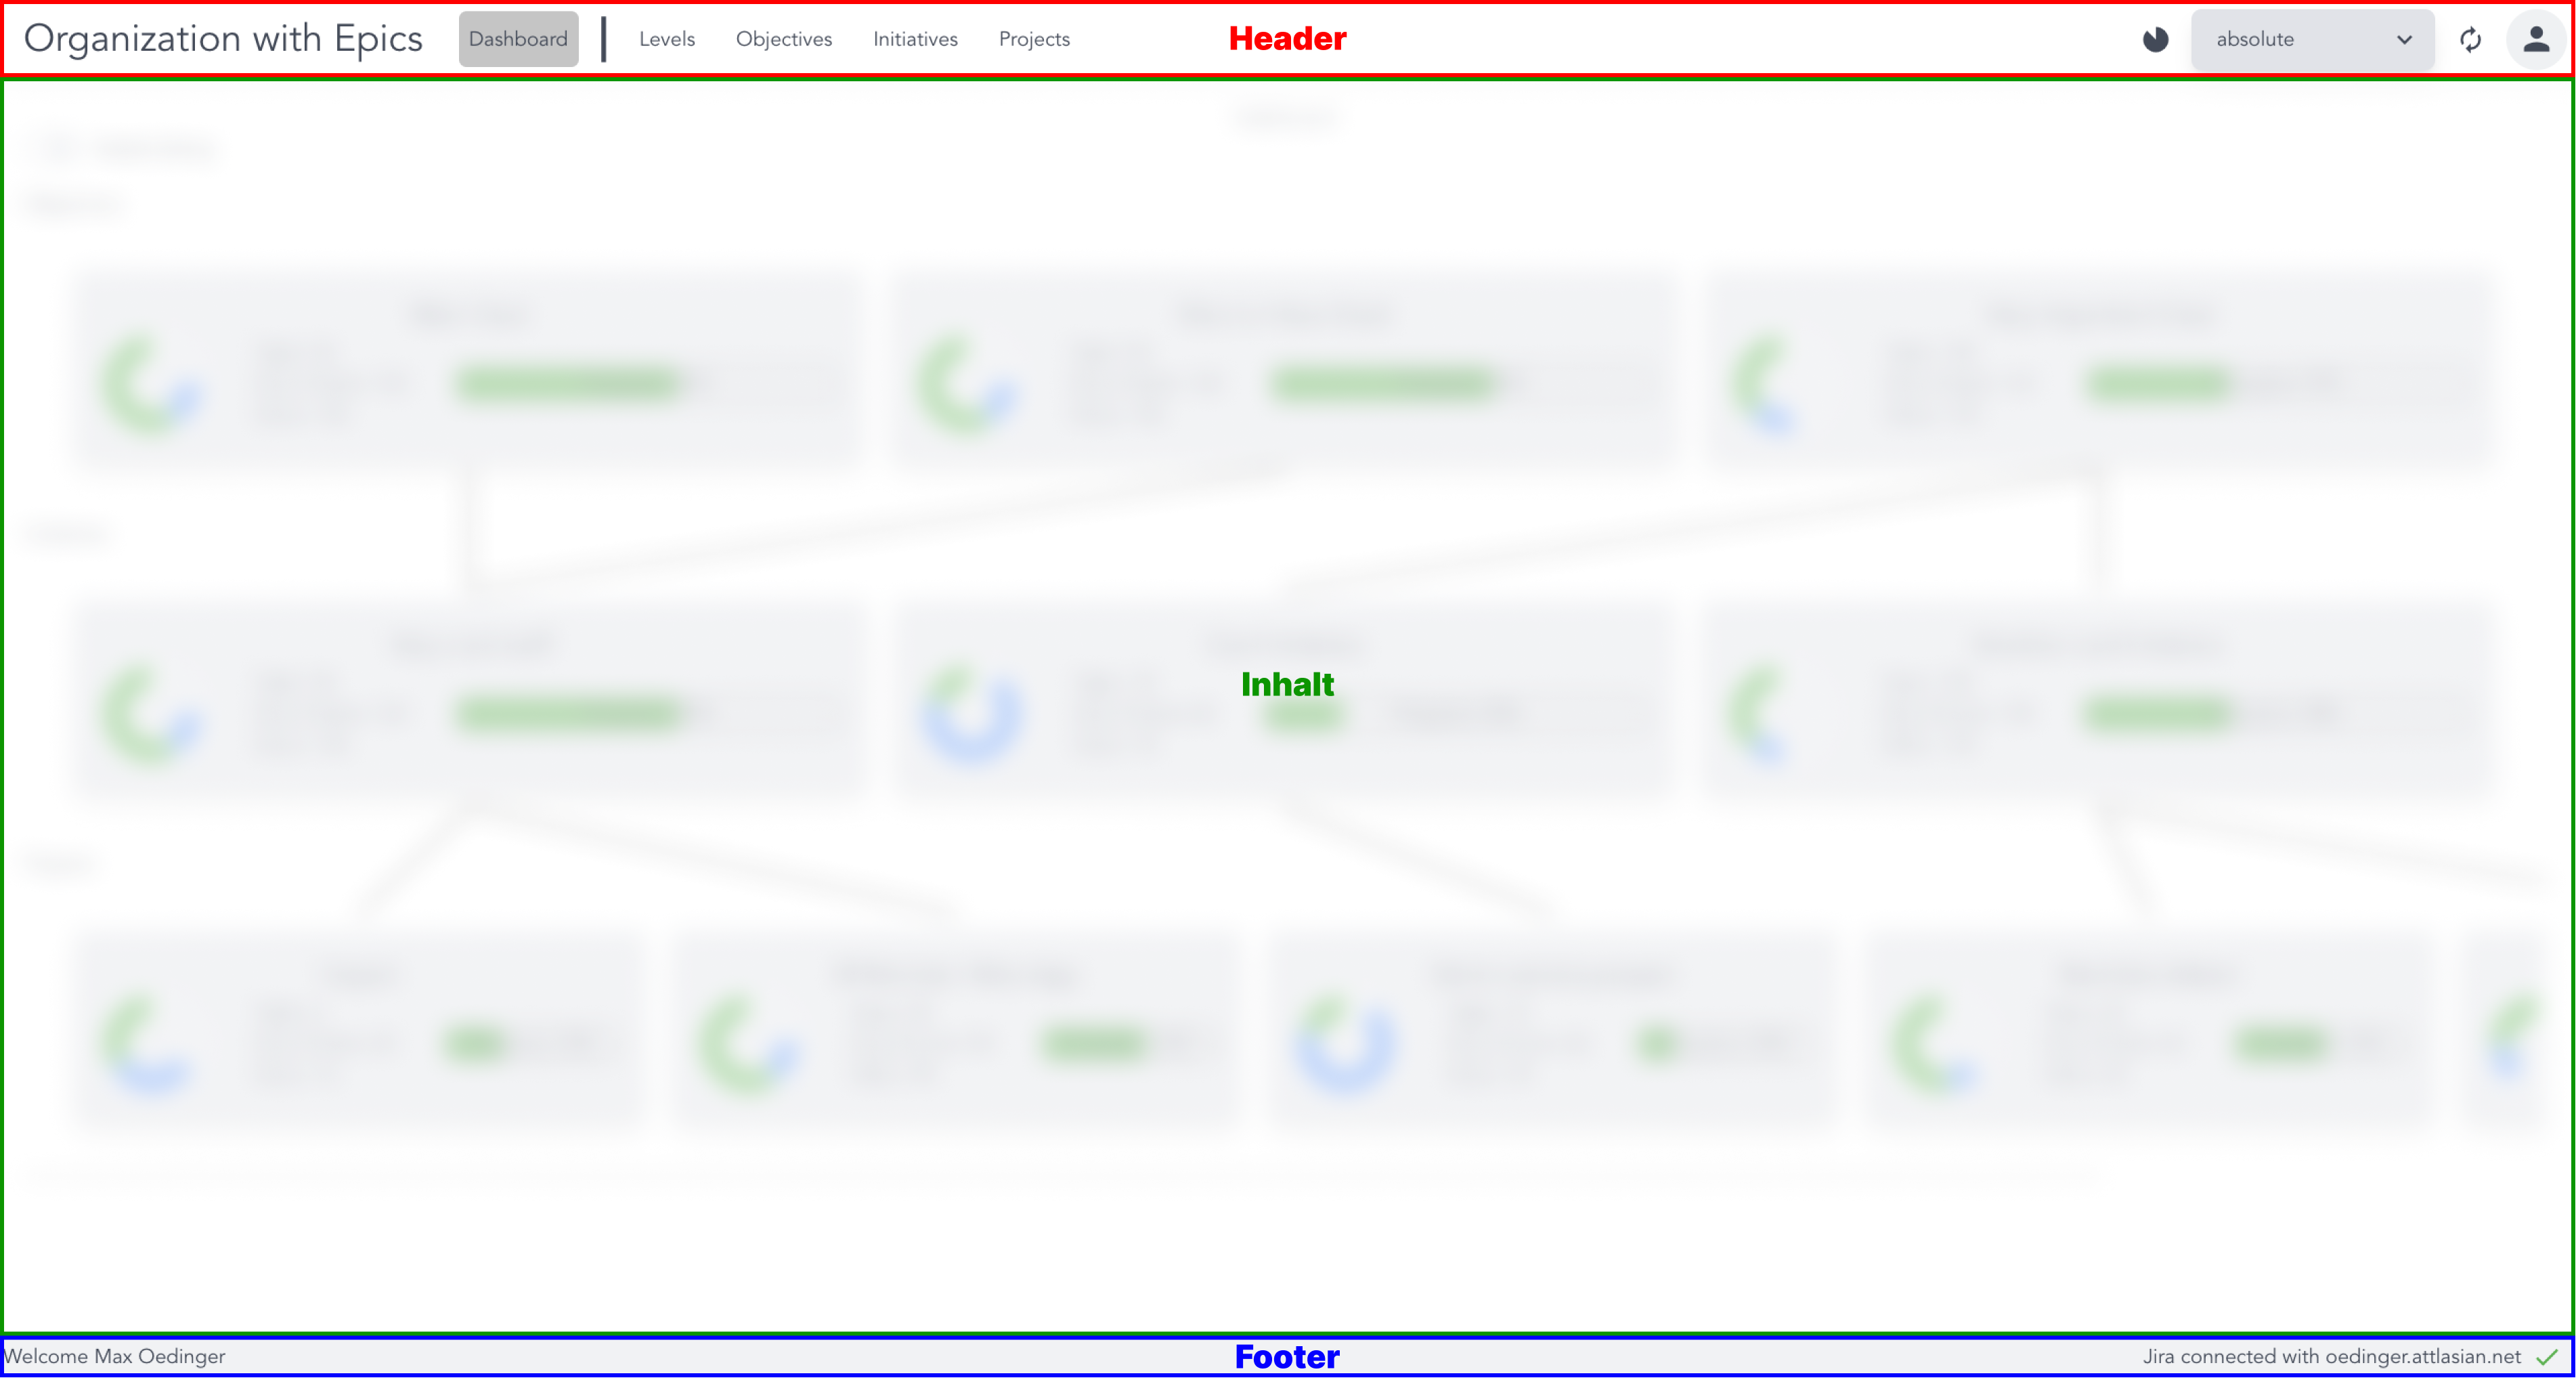
\includegraphics[width=\linewidth]{mainLayout}
        \captionof{figure}{Visualisierung des Layouts}
    \end{minipage}
\end{center}
\vspace{20pt}

Das Layout der eigentlichen Seite teilt die Seite in drei Teile, den Header, den Inhalt und einen Footer. Der Header beinhaltet die Navigationsleiste, die den Nutzer durch die Anwendung führt und oben rechts ein Aktionsmenü mit dem der Nutzer sich jederzeit ausloggen kann oder in die Einstellungen bzw. sein Profil navigieren kann. Zudem kann der Nutzer links neben dem Aktionsmenü die Daten der Anwendung erneut laden und die Fortschrittsmessung zwischen Absolut, Storypoints und Value auswählen. Der Inhalt ist der Bereich in dem die verschiedenen Views dargestellt werden. Im Footer sind Informationen über den aktuell eingeloggten Nutzer und seine Verbindung zu Jira enthalten.

\subsubsection{Views und Components}
Die Views beinhalten die im UX-Entwurf beschriebenen Anwendungsteile: Login, Registrierung, Passwort vergessen, Passwort Reset, Dashboard, Einstellungen, Profil, Organisationen, Level-Übersicht, Gruppenansicht, Gruppendetailansicht, Projektübersicht, Projekt-Dashboard, Aufgaben-Board, Aufgaben-Backlog und Epic-Übersicht. Außerdem gibt es eine Not-Found-View welche dargestellt wird, wenn der Nutzer versucht eine nicht existierende Seite aufzurufen und eine Home-View, die als Homepage der Anwendung dient. Hier kann der Nutzer das Dokument der Bachelorarbeit sehen und die API-Dokumentation aufrufen.

Die Components enthalten mehrfach verwendetet UI-Elemente, wie z. B. Buttons, Icons, Textfelder, Dropdowns, Drag-And-Drop-Elemente, Dialogfenster, etc.


\subsubsection{Datenverwaltung}
Für die anwendungsübergreifende Datenverwaltung wird das Framework Pinia als Store verwendet. Der Store dient dazu die Daten nicht kontextspezifisch zu speichern, sondern in der gesamten Anwendung verfügbar zu machen. Somit müssen die Daten nicht nach jeden Seitenwechsel neu geladen werden, sondern können aus dem Store abgerufen werden. Dies verbessert die Performance der Anwendung. Außerdem werden alle Kommunikationen mit dem Backend über den Store abgewickelt und durch die Ergebnisse der Kommunikationen werden die Daten im Store aktualisiert. Daten, die aus dem Store abgerufen werden, sind reactive, das bedeutet, dass Änderungen der Daten ebenfalls in den Komponenten, welche die Daten verwenden, reflektiert werden. Ein Store besteht aus drei verschiedenen Teilen: State, Getters und Actions. Der State beschreibt den Zustand der Daten. Getters sind Funktionen, die Daten aus dem State für verschiedene Anwendungsfälle transformiert oder gefiltert zurückgeben. Actions sind Funktionen, welche die Kommunikation mit dem Backend abwickeln und mit den zurückgegebenen Daten den State mutieren.

Es gibt mehrere Stores, die verschiedene Daten speichern. Für allgemeine Informationen gibt es den AppStore. Diese speichert welche Fortschrittsmessung ausgewählt wurde und ob der Light- oder Darkmode ausgewählt wurde. Der AppStore wird zusätzlich im Local-Storage des Browsers persistiert, was dafür sorgt, dass diese Informationen auch bei einem Neuladen der Seite erhalten bleiben.

Im AuthStore wird der eingeloggte Nutzer gespeichert und ob der Nutzer eingeloggt ist und Login und Logout definiert.
Für Daten, die in der Backend- und Datenstruktur als Entitäten bezeichnet werden gibt es auch hier eine Abstraktion der Stores für die Verwaltung dieser Entitäten. Es gibt also auch hier eine Abstraktion in EntityStore, OrganizationBasedEntity und LinkableEntity, von welchen die tatsächlich verwendeten Stores für die verschiedenen Datentypen erben. Anders als die Backendstruktur funktioniert die Vererbung hier aber nicht über Klassen, da Pinia einem funktionalen Implementierungsschema folgt. Also gibt es MakeFunktionen für jedes der drei verschiedenen Teile des Stores, welche mit Generischen-Type-Parametern State, Getter und Actions mit den richtigen Typen erzeugt. Für simple Stores wie z. B. den OrganizationStore beschränkt sich die absolute Implementierung dann wie folgt:

\begin{lstlisting}[language=JavaScript, caption=Implementierung des OrganizationStores]
export const useOrganizationStore: EntityStoreDefinition<
    IOrganization,
    'organization'
> = defineStore('organization', {
    state: makeEntityState<IOrganization>(organizationService),
    getters: makeEntityGetters<IOrganization>(),
    actions: makeEntityActions<IOrganization>(),
});
\end{lstlisting}

Für Stores mit zusätzlichen Getters, werden die MakeFunktionen erweitert, wie beispielsweise im LevelStore:

\begin{lstlisting}[language=JavaScript, caption=Implementierung des LevelStores]
interface LevelGetters extends OrganizationBasedEntityGetters<ILevel> {
    getNextHierarchyLevel(): number;
    isProjectLevel(): (levelId: string) => boolean;
    getLowerLevel(): Level | undefined;
}

type LevelStore = OrganizationBasedEntityStore<
    ILevel,
    'level',
    OrganizationBasedEntityState<ILevel>,
    LevelGetters
>;
type LevelStoreDefinition = OrganizationBasedEntityStoreDefinition<
    ILevel,
    'level',
    OrganizationBasedEntityState<ILevel>,
    LevelGetters
>;

const levelStore: PiniaStore<LevelStore> = {
    state: makeOrganizationBasedEntityState<ILevel>(levelService),
    getters: {
        ...makeOrganizationBasedEntityGetters<ILevel>(),
        getNextHierarchyLevel(state) {
            const currentOrganization = useOrganizationStore().currentEntity;
            if (!currentOrganization) return 0;
            return state.entities.filter(
                ({ organizationId }) => organizationId === currentOrganization.id
            ).length;
        },
        isProjectLevel(state) {
            return (levelId: string) => {
                const projectLevel = useOrganizationStore().currentEntity?.useEpics
                    ? 1
                    : 0;
                return (
                    state.entities.find((level) => level.id === levelId)
                        ?.hierarchyLevel === projectLevel
                );
            };
        },
        getLowerLevel(state) {
            const currentLevel: Entity<OrganizationBasedEntity<ILevel>> =
                state.currentEntity;
            if (!currentLevel) return;

            return state.entities.find(
                (x) =>
                    x.organizationId === currentLevel.organizationId &&
                    x.hierarchyLevel === currentLevel.hierarchyLevel - 1
            );
        },
    },
    actions: makeOrganizationBasedEntityActions<ILevel>(),
};

export const useLevelStore: LevelStoreDefinition = defineStore(
    'level',
    levelStore
);
\end{lstlisting}

Stores für Entitäten, haben in ihrem State zusätzlich ein Loaded Attribut in dem gespeichert wird, ob die Daten bereits von Server abgefragt wurde, bzw. wenn es sich um eine OrganizationBasedEntity handelt, ob die Daten für diese Organisation bereits geladen wurde, um mehrfache Requests für die gleichen Daten zu vermeiden und damit die Performance zu verbessern.

Der Jira-Store speichert alle den Nutzer zugänglichen Projekte und bietet mit seinen Actions die Möglichkeit die relevanten Daten zu diesem Projekt zu holen, wenn der Nutzer den Import-Prozess für ein Jira-Projekt startet.

\subsection{Projekt-Import}
Um die Verwendung der Anwendung zu vereinfachen, wurde ein Import-Prozess sowohl für Projektdaten in Excel-Dateien, als auch für Jira-Projekte implementiert. Projekte, welche eine große Menge an Daten beinhalten und in meist in externen Tools dokumentiert und verwaltet werden, können somit ohne größeren Aufwand in der Anwendung verwendet werden. Dieser Import Prozess erlaubt ein individuelles Mapping der Daten aus den externen Tools auf die Datenstruktur der Anwendung. Das Mapping bei einer Excel-Tabelle erwartet eine Excel-Tabelle, welche alle Aufgaben eines Projekts enthält. Hierbei kann der Nutzer  die Felder aus der Anwendung mit Drag-and-Drop Spalten in der Tabelle zuordnen. Sollten Spalten die gleiche Bezeichnung wie Felder innerhalb der Anwendung haben, werden diese Felder automatisch zugeordnet. Diese automatischen Zuordnungen können vom Nutzer wieder abgeändert werden.

\vspace{20pt}
\begin{center}
    \begin{minipage}{1\linewidth}
        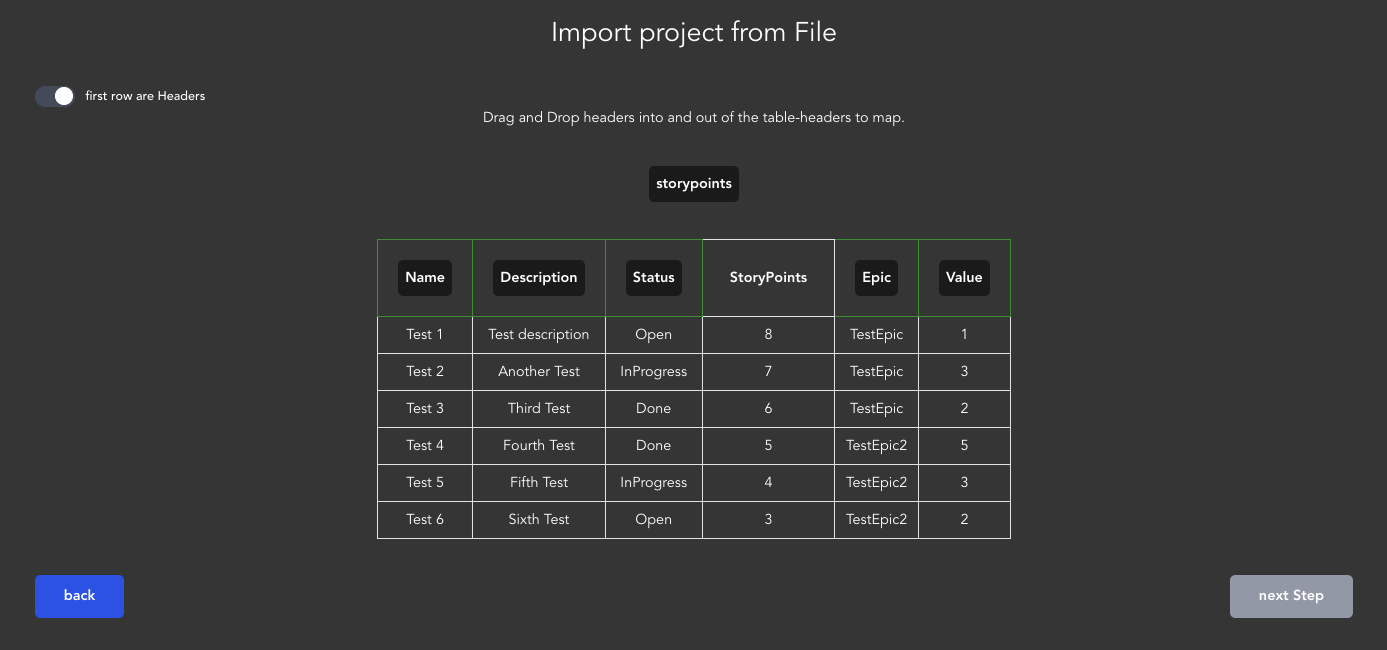
\includegraphics[width=\linewidth]{ImportExcel}
        \captionof{figure}{Import Feld Mapping}
    \end{minipage}
\end{center}
\vspace{20pt}

Anschließend wird für das Feld, welches den Status der Aufgabe enthält, einem Status innerhalb der Anwendung zuordnen. Enthält das Feld für eine Aufgabe den gleichen Wert wie der zugeordnete Status, wird dieser verwendet.

\vspace{20pt}
\begin{center}
    \begin{minipage}{1\linewidth}
        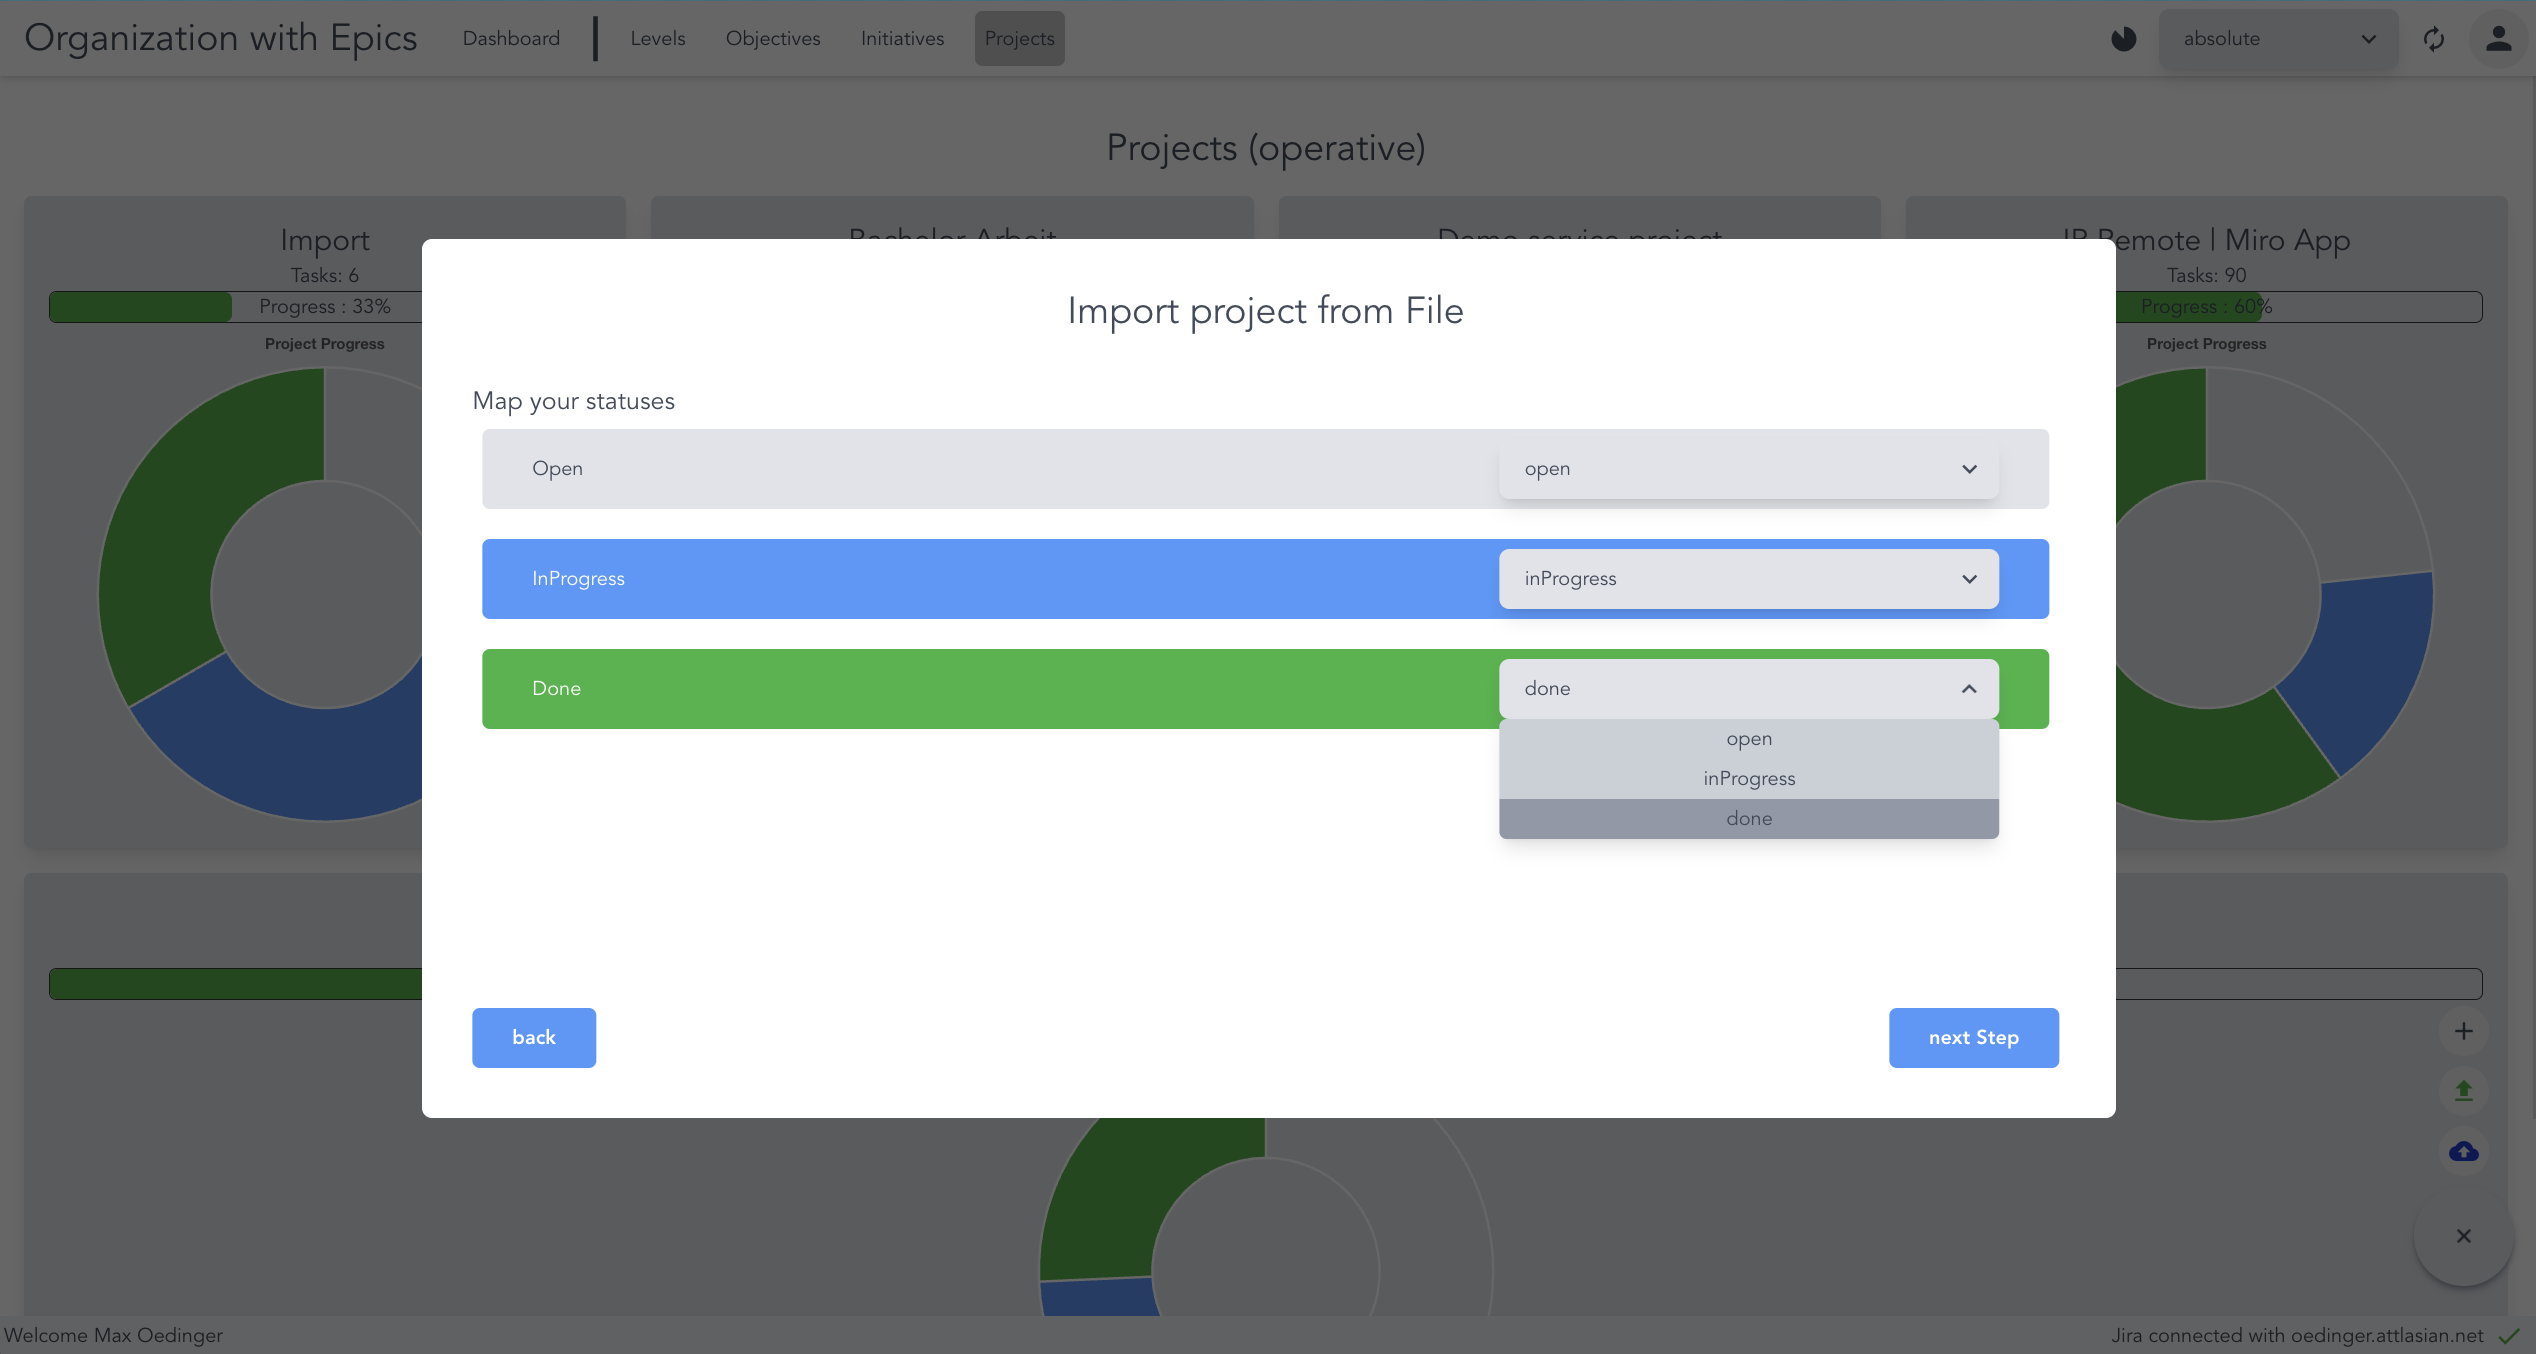
\includegraphics[width=\linewidth]{ImportStatusMapping}
        \captionof{figure}{Import Status Mapping}
    \end{minipage}
\end{center}
\vspace{20pt}

Importiert der Nutzer von Jira kann er zunächst ein Projekt auswählen.

\vspace{20pt}
\begin{center}
    \begin{minipage}{1\linewidth}
        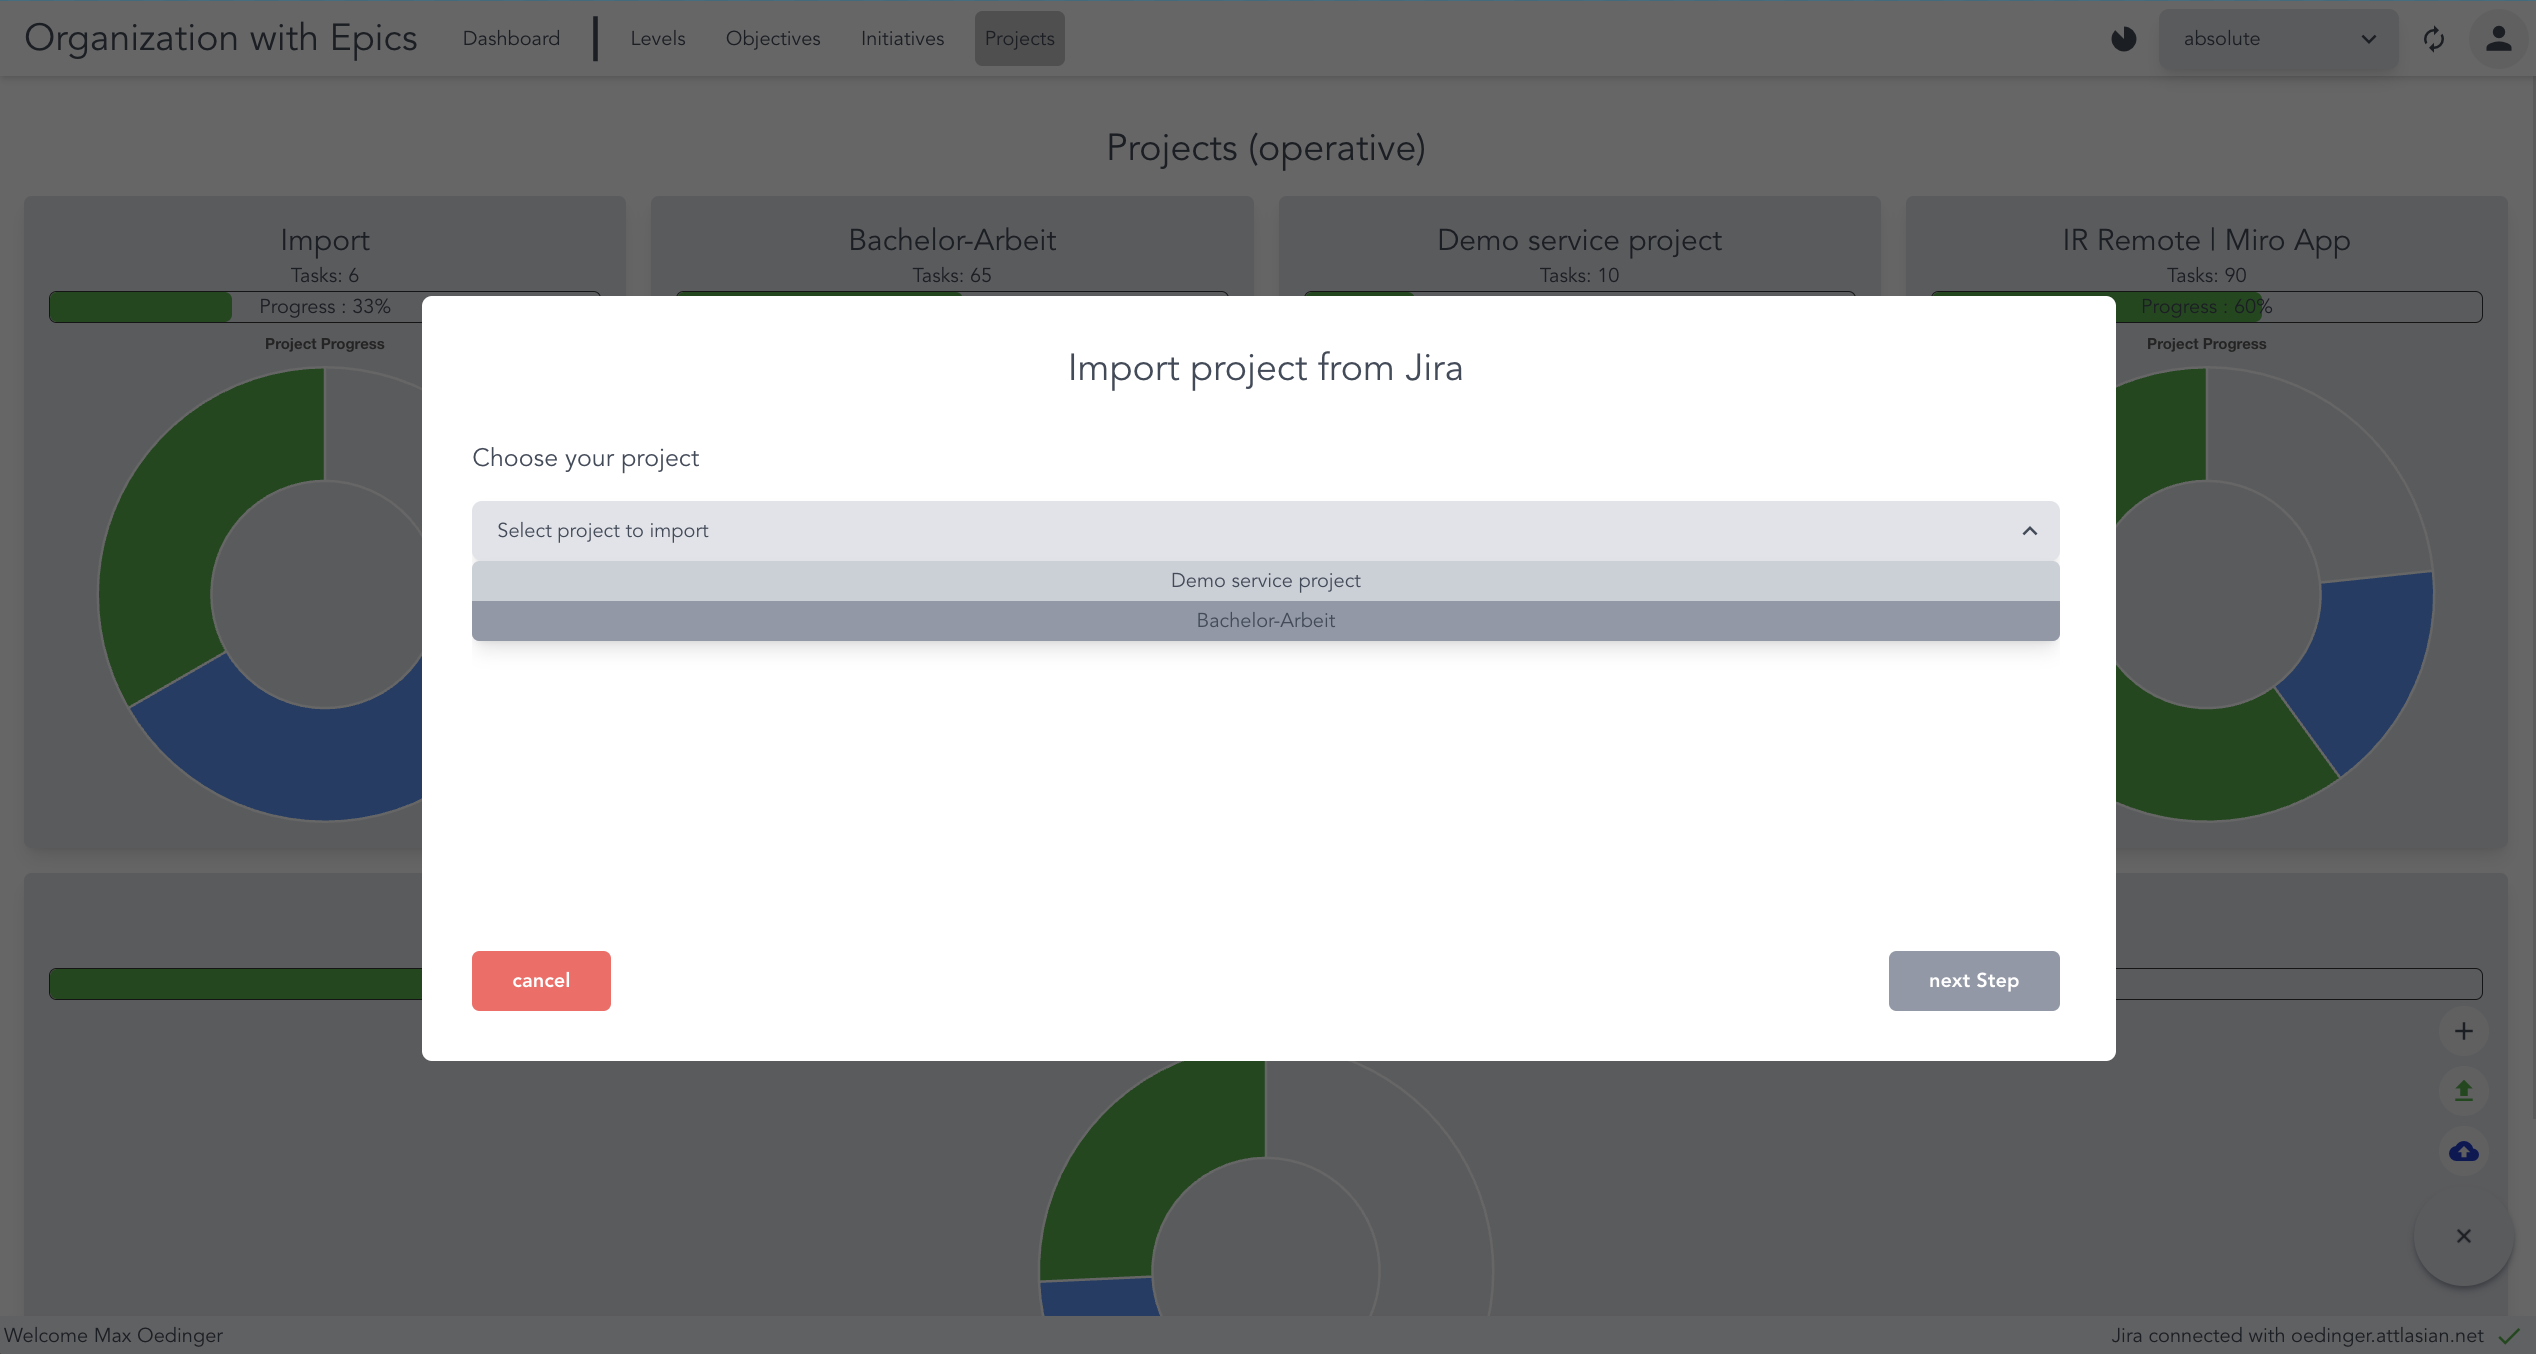
\includegraphics[width=\linewidth]{ImportJiraProjectSelection}
        \captionof{figure}{Import Jira Projekt Auswahl}
    \end{minipage}
\end{center}
\vspace{20pt}

\vspace{20pt}
\begin{center}
    \begin{minipage}{1\linewidth}
        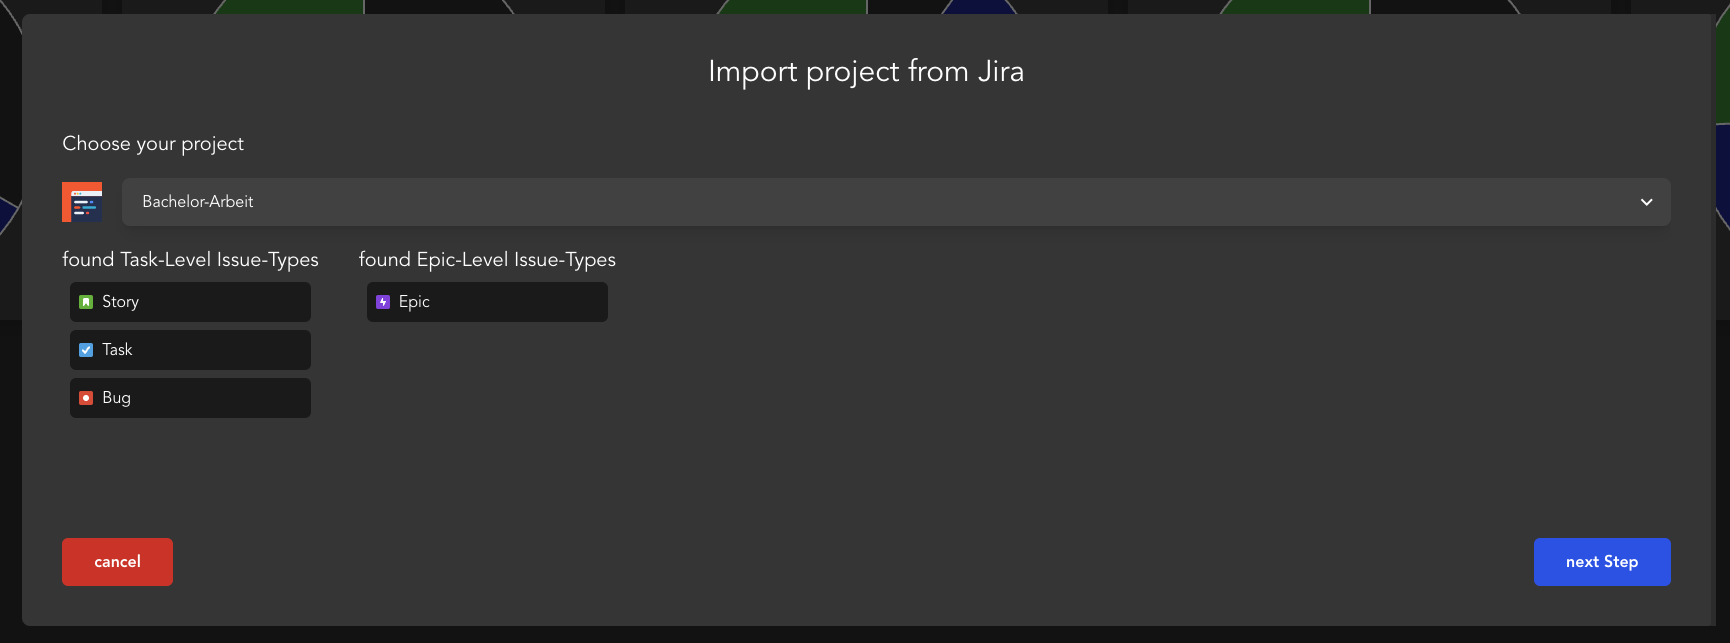
\includegraphics[width=\linewidth]{ImportJiraProjectSelected}
        \captionof{figure}{Import Jira Ansicht nach Projekt Auswahl}
    \end{minipage}
\end{center}
\vspace{20pt}

Für Jira-Projekte kann das Mapping der Felder größtenteils automatisch durchgeführt werden, das bedeutet, dass Aufgaben und Epics sofort erkannt werden. Die Stati der Aufgaben können anhand der Metadaten von JIRA auch automatisch ausgelesen werden, der Nutzer kann dennoch Für jeden Status aus JIRA ändern, welcher Status im Prototypen zugeordnet wird, falls die tatsächliche Verwendung von den Meta-Daten abweichen sollte.

\vspace{20pt}
\begin{center}
    \begin{minipage}{1\linewidth}
        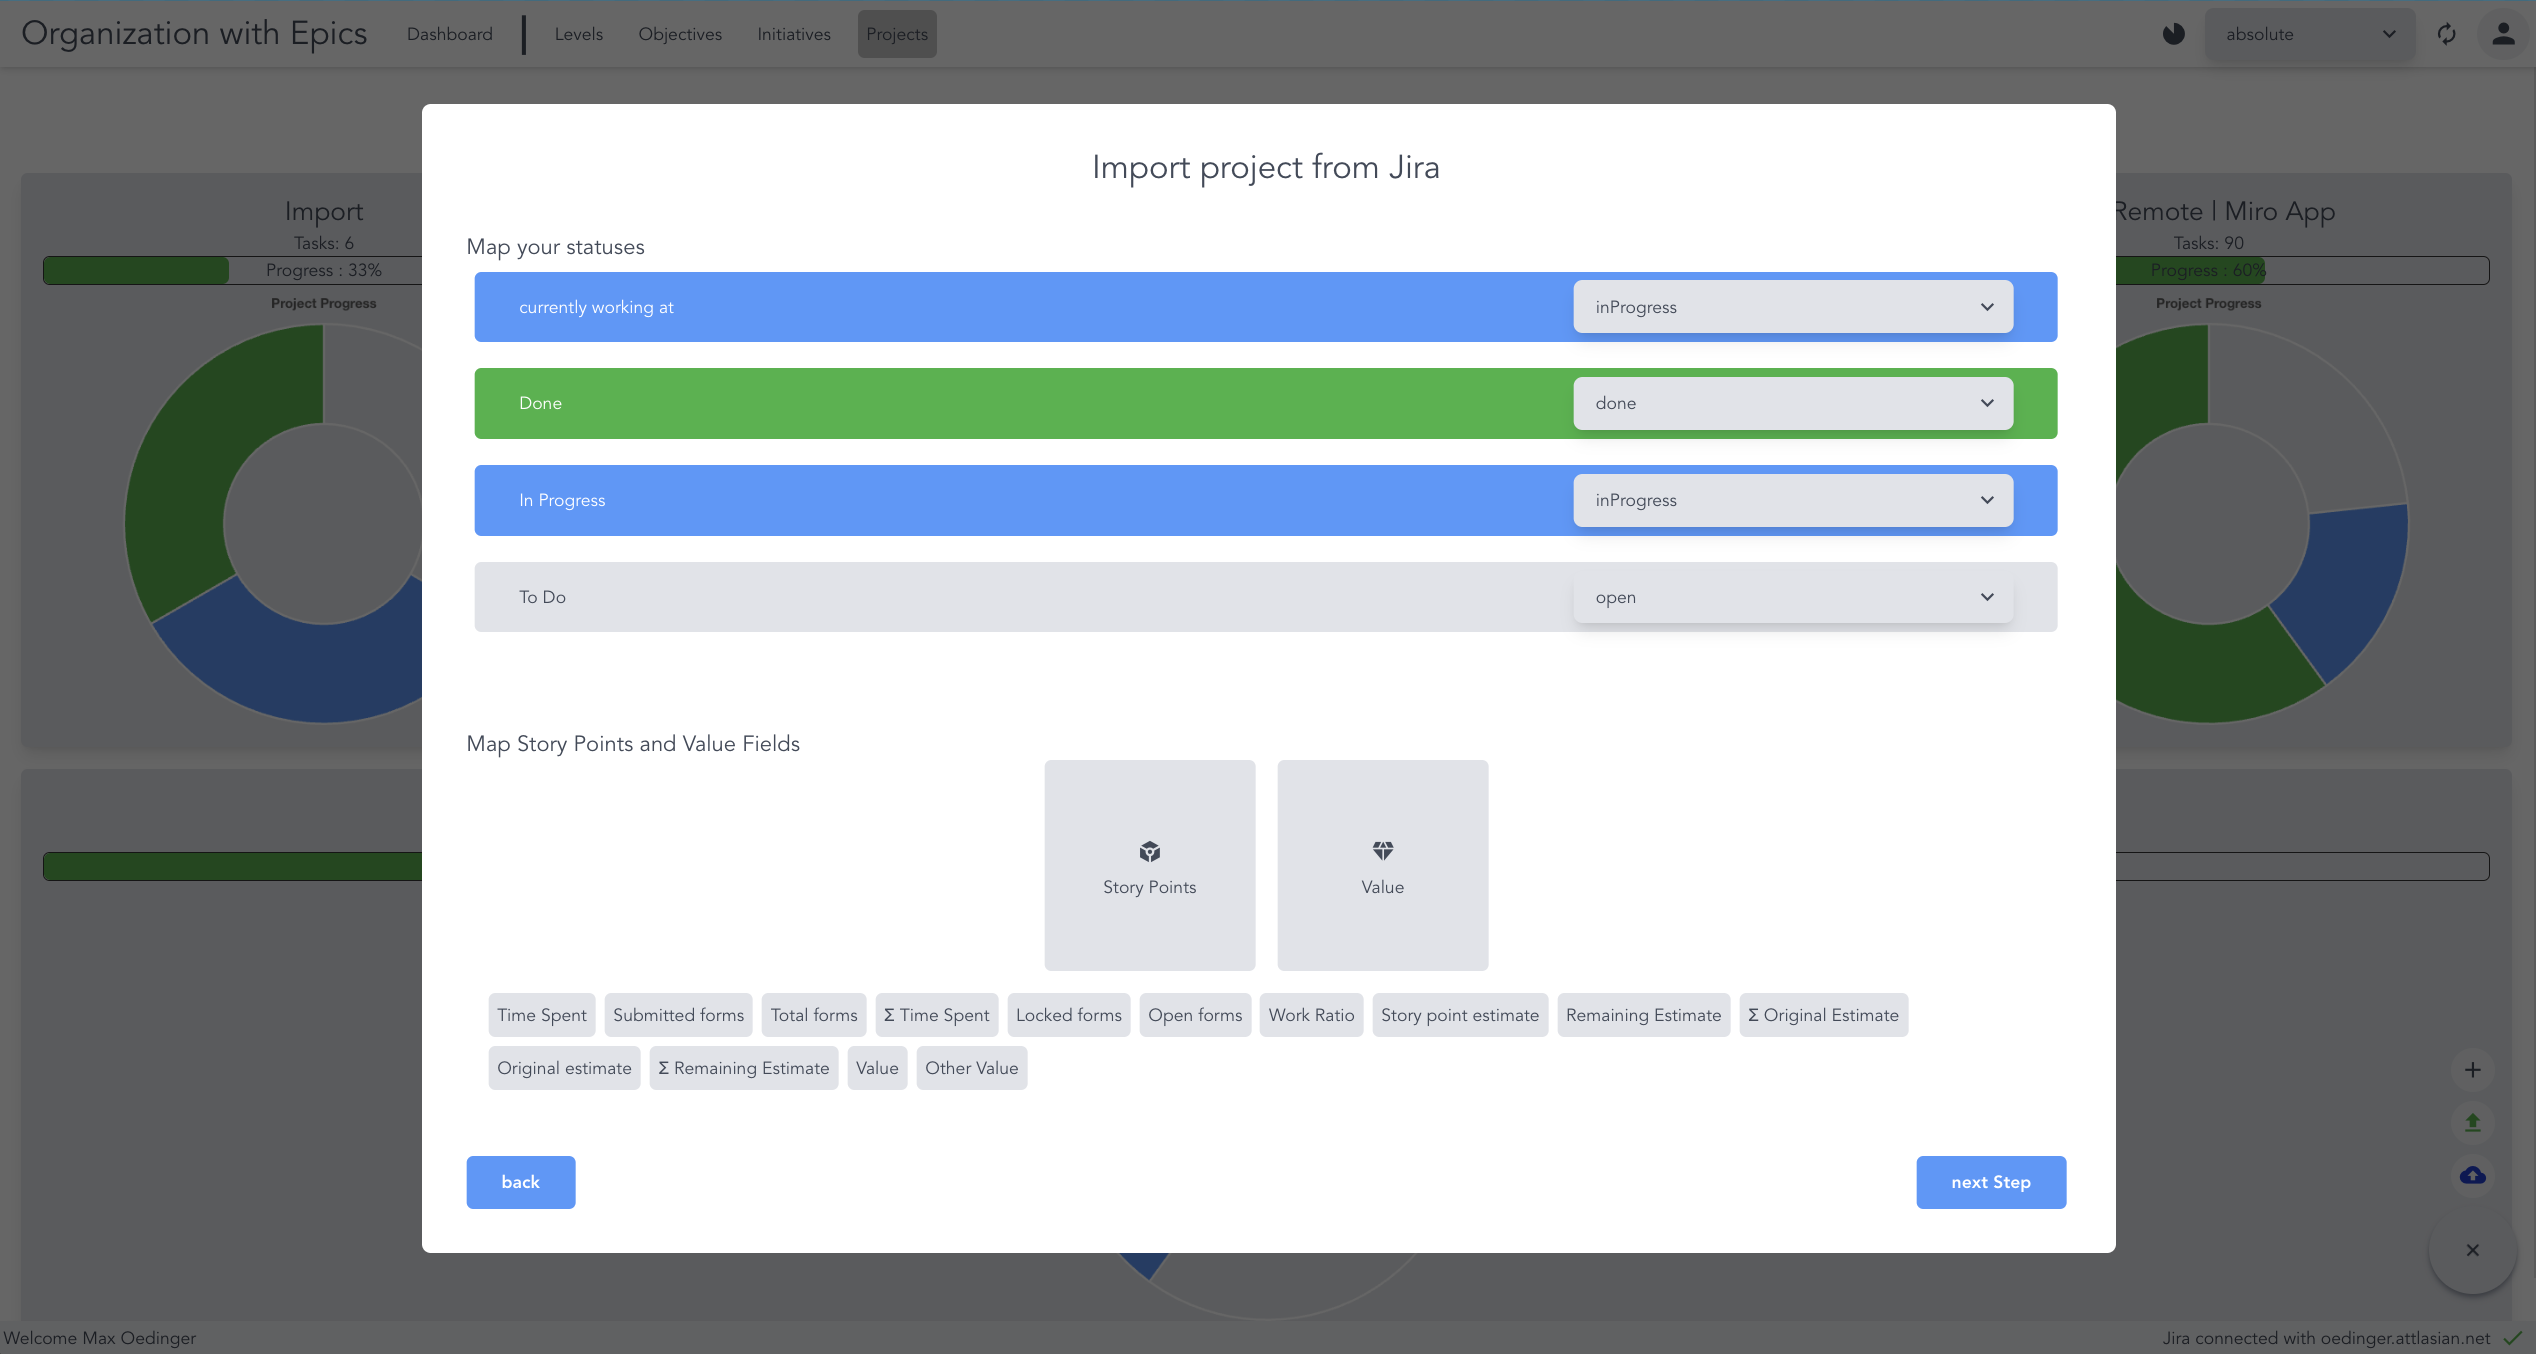
\includegraphics[width=\linewidth]{ImportJiraMapping}
        \captionof{figure}{Import Jira Mapping}
    \end{minipage}
\end{center}
\vspace{20pt}

Außerdem kann der Nutzer an dieser Stelle Custom-Fields für Issues aus Jira, welche Zahlenwerte enthalten auf Value und/oder Storypoints mappen.

Zuletzt erhält der Nutzer nocheinmal eine Übersicht über die importierten Daten und kann den Import-Prozess starten.

\vspace{20pt}
\begin{center}
    \begin{minipage}{1\linewidth}
        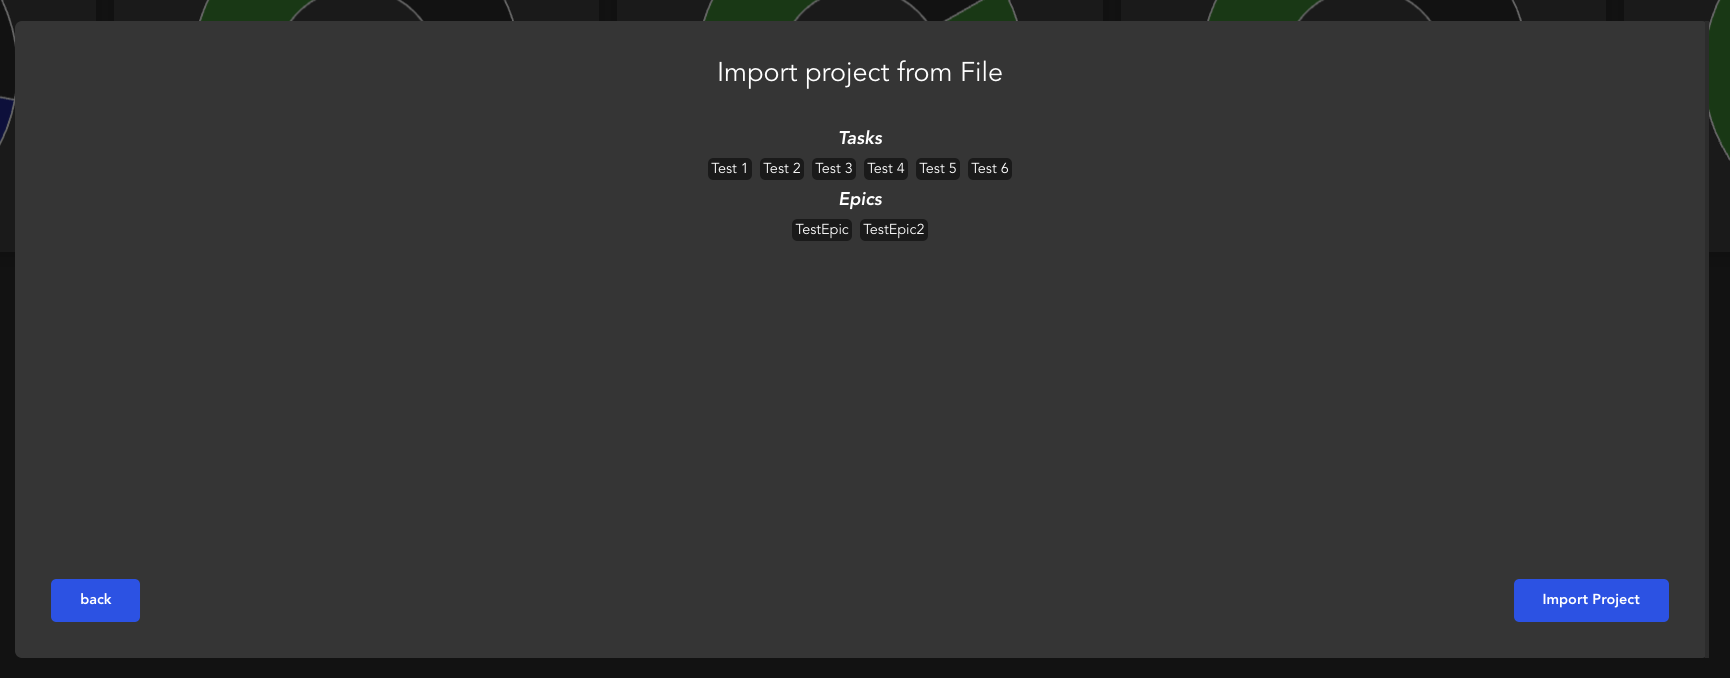
\includegraphics[width=\linewidth]{ImportUebersicht}
        \captionof{figure}{Import Übersicht bei Excel Datei}
    \end{minipage}
\end{center}
\vspace{20pt}

\vspace{20pt}
\begin{center}
    \begin{minipage}{1\linewidth}
        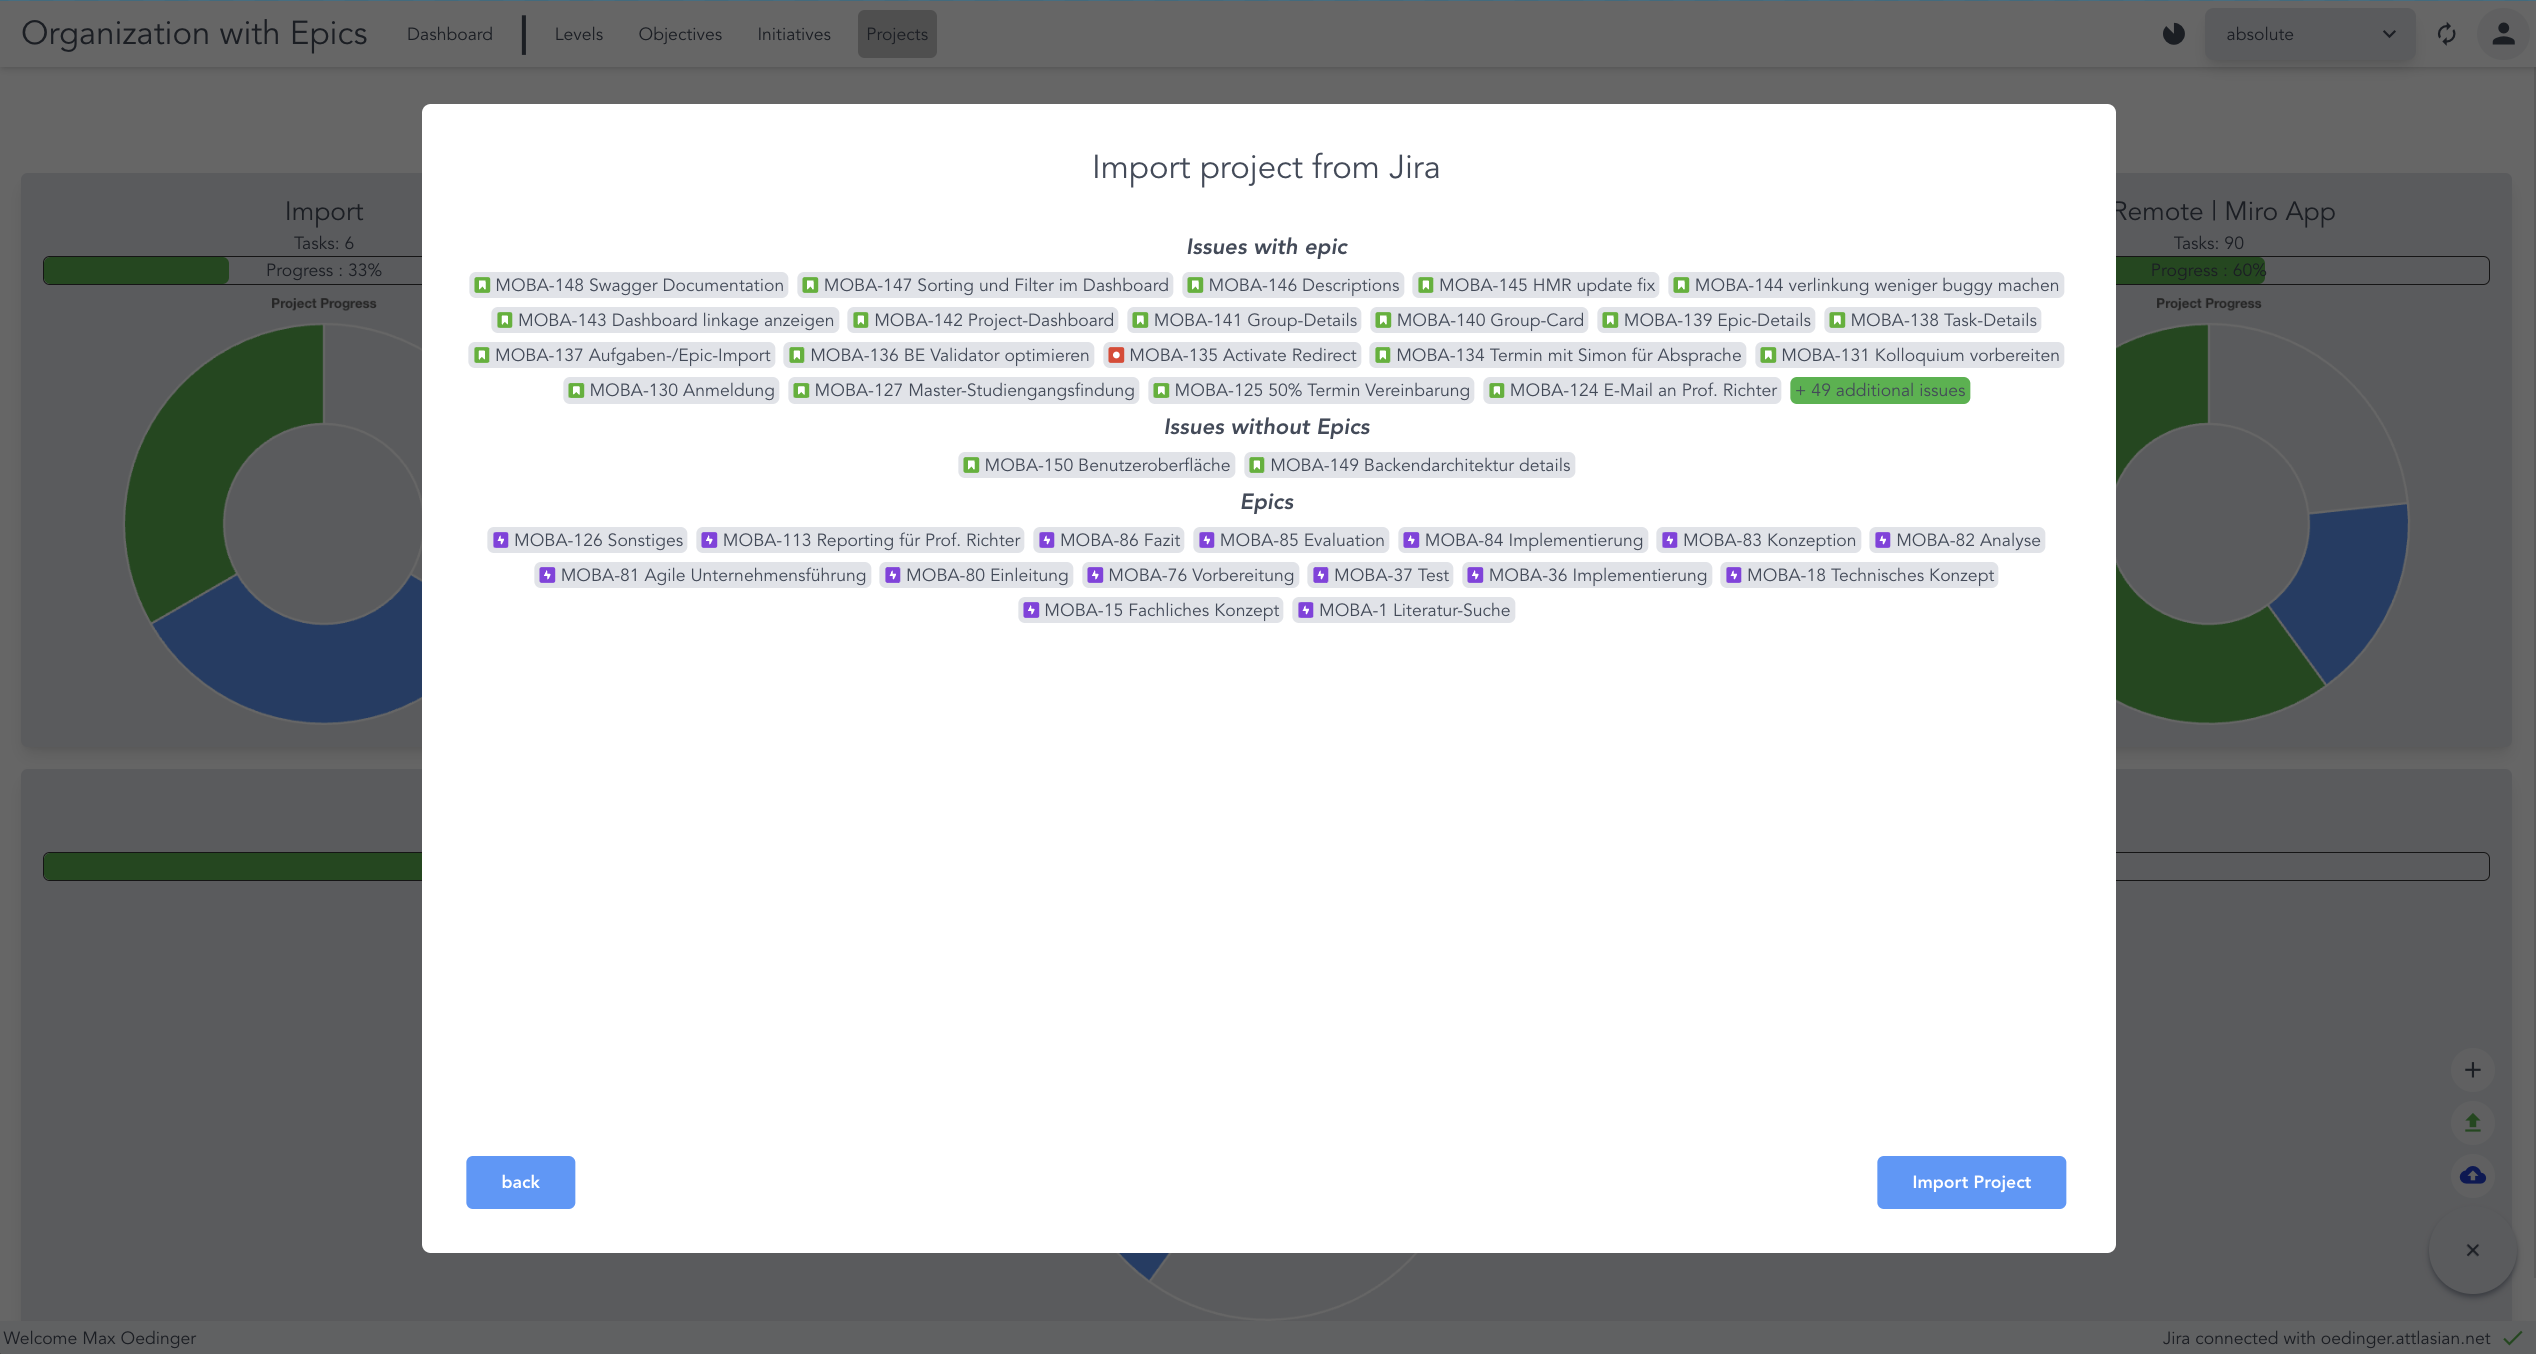
\includegraphics[width=\linewidth]{ImportJiraUebersicht}
        \captionof{figure}{Import Übersicht bei Jira Import}
    \end{minipage}
\end{center}
\vspace{20pt}

\subsection{Visualisierung/Datendarstellung}
Für die generelle Visualisierung der gesamten Daten einer Organisation dient das Dashboard, welches den komplexesten Teil der Anwendung darstellt.

Hier werden alle Gruppen der Organisation hierarchisch sortiert dargestellt und ihre Verknüpfungen untereinander visualisiert.
Um die Übersicht bei vielen Gruppen beizubehalten werden die Gruppen innerhalb einer hierarchischen Ebene nach ihren Verbindungen zu den darüberliegenden Gruppen sortiert, sodass Gruppen, die mit der gleichen Gruppe in der Ebene darüber verknüpft sind, nebeneinander dargestellt werden. Die Verbindungslinien werden somit möglichst kurz und übersichtlich dargestellt.

\vspace{20pt}
\begin{center}
    \begin{minipage}{1\linewidth}
        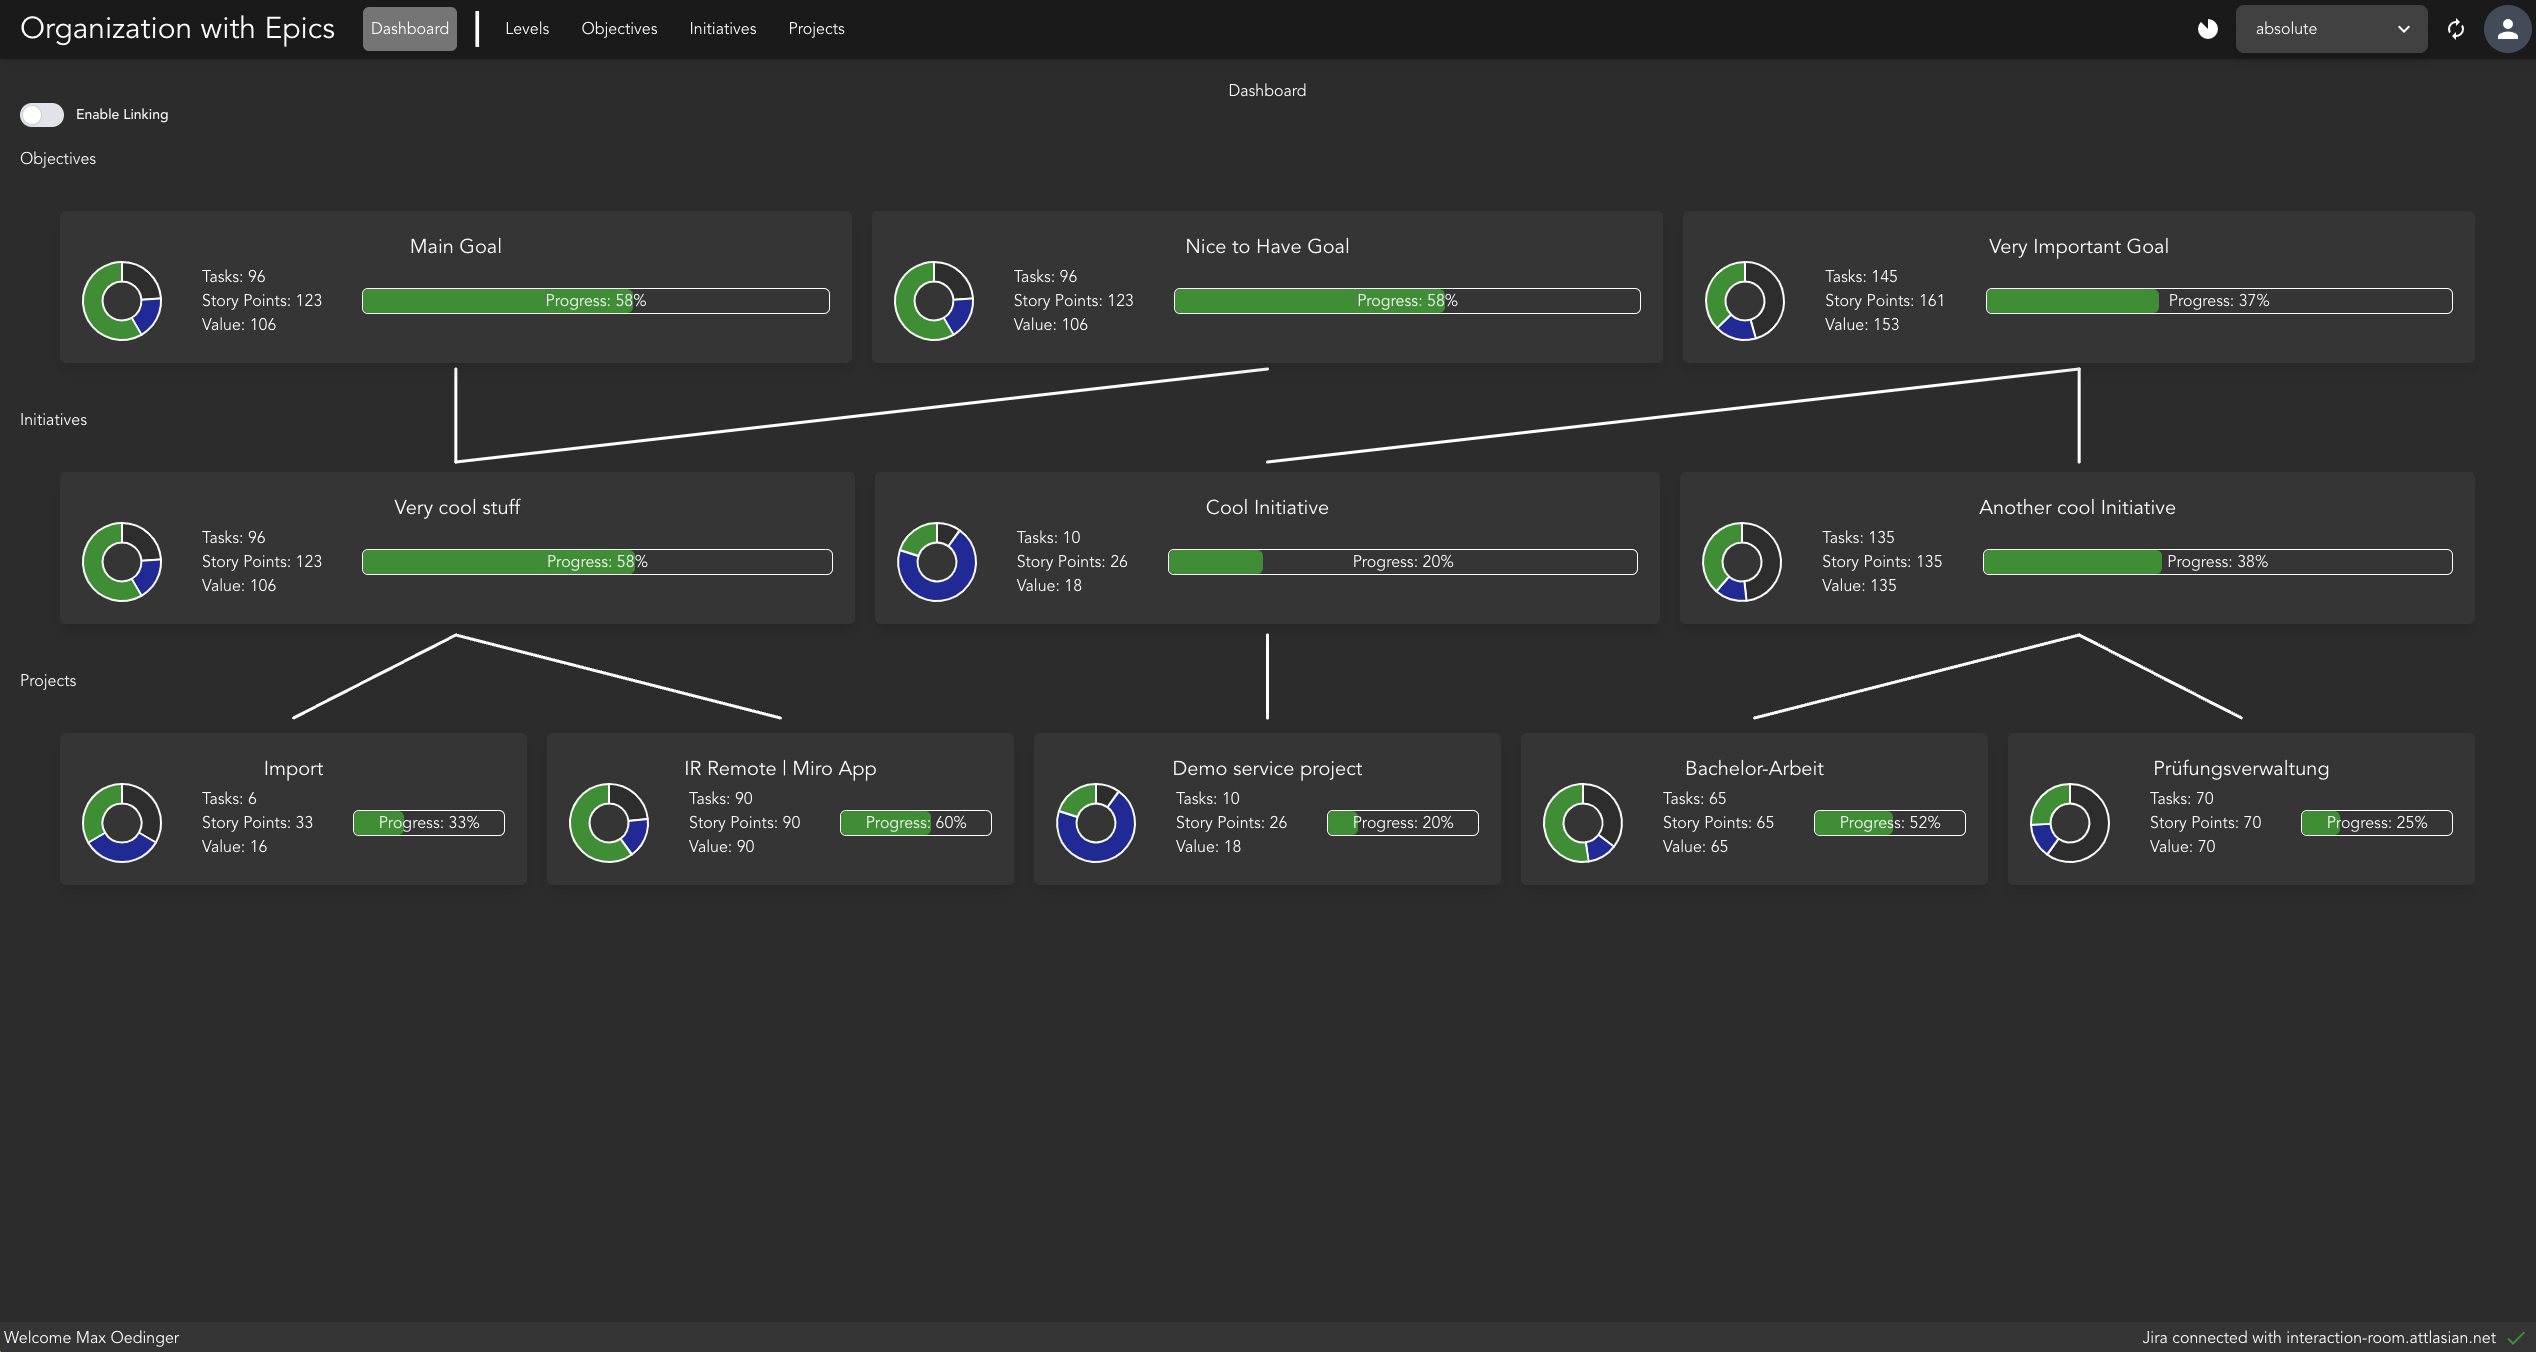
\includegraphics[width=\linewidth]{Dashboard_full}
        \captionof{figure}{Dashboard}
    \end{minipage}
\end{center}
\vspace{20pt}

Um die Verbindungslinien darzustellen wurde ein SVG-Element im Hintergrund der Seite verwendet, welches die Verbindungslinien unabhängig von anderen Elementen auf der Seite darstellen kann. Die Start- und Endkoordinaten der Linien werden durch Positionen der Gruppen innerhalb der Seite berechnet. Dabei muss zusätzlich beachtet werden, wenn ein Level so viele Gruppen beinhaltet, dass sich einige Gruppen außerhalb des sichtbaren Bereichs befinden können. Durch Scrollen können sie in den sichtbaren Bereich bewegt werden. In diesem Fall müssen die Koordinaten der Linien entsprechend der Scroll-Position der verschobenen Gruppen neu berechnet werden.

\vspace{20pt}
\begin{center}
    \begin{minipage}{1\linewidth}
        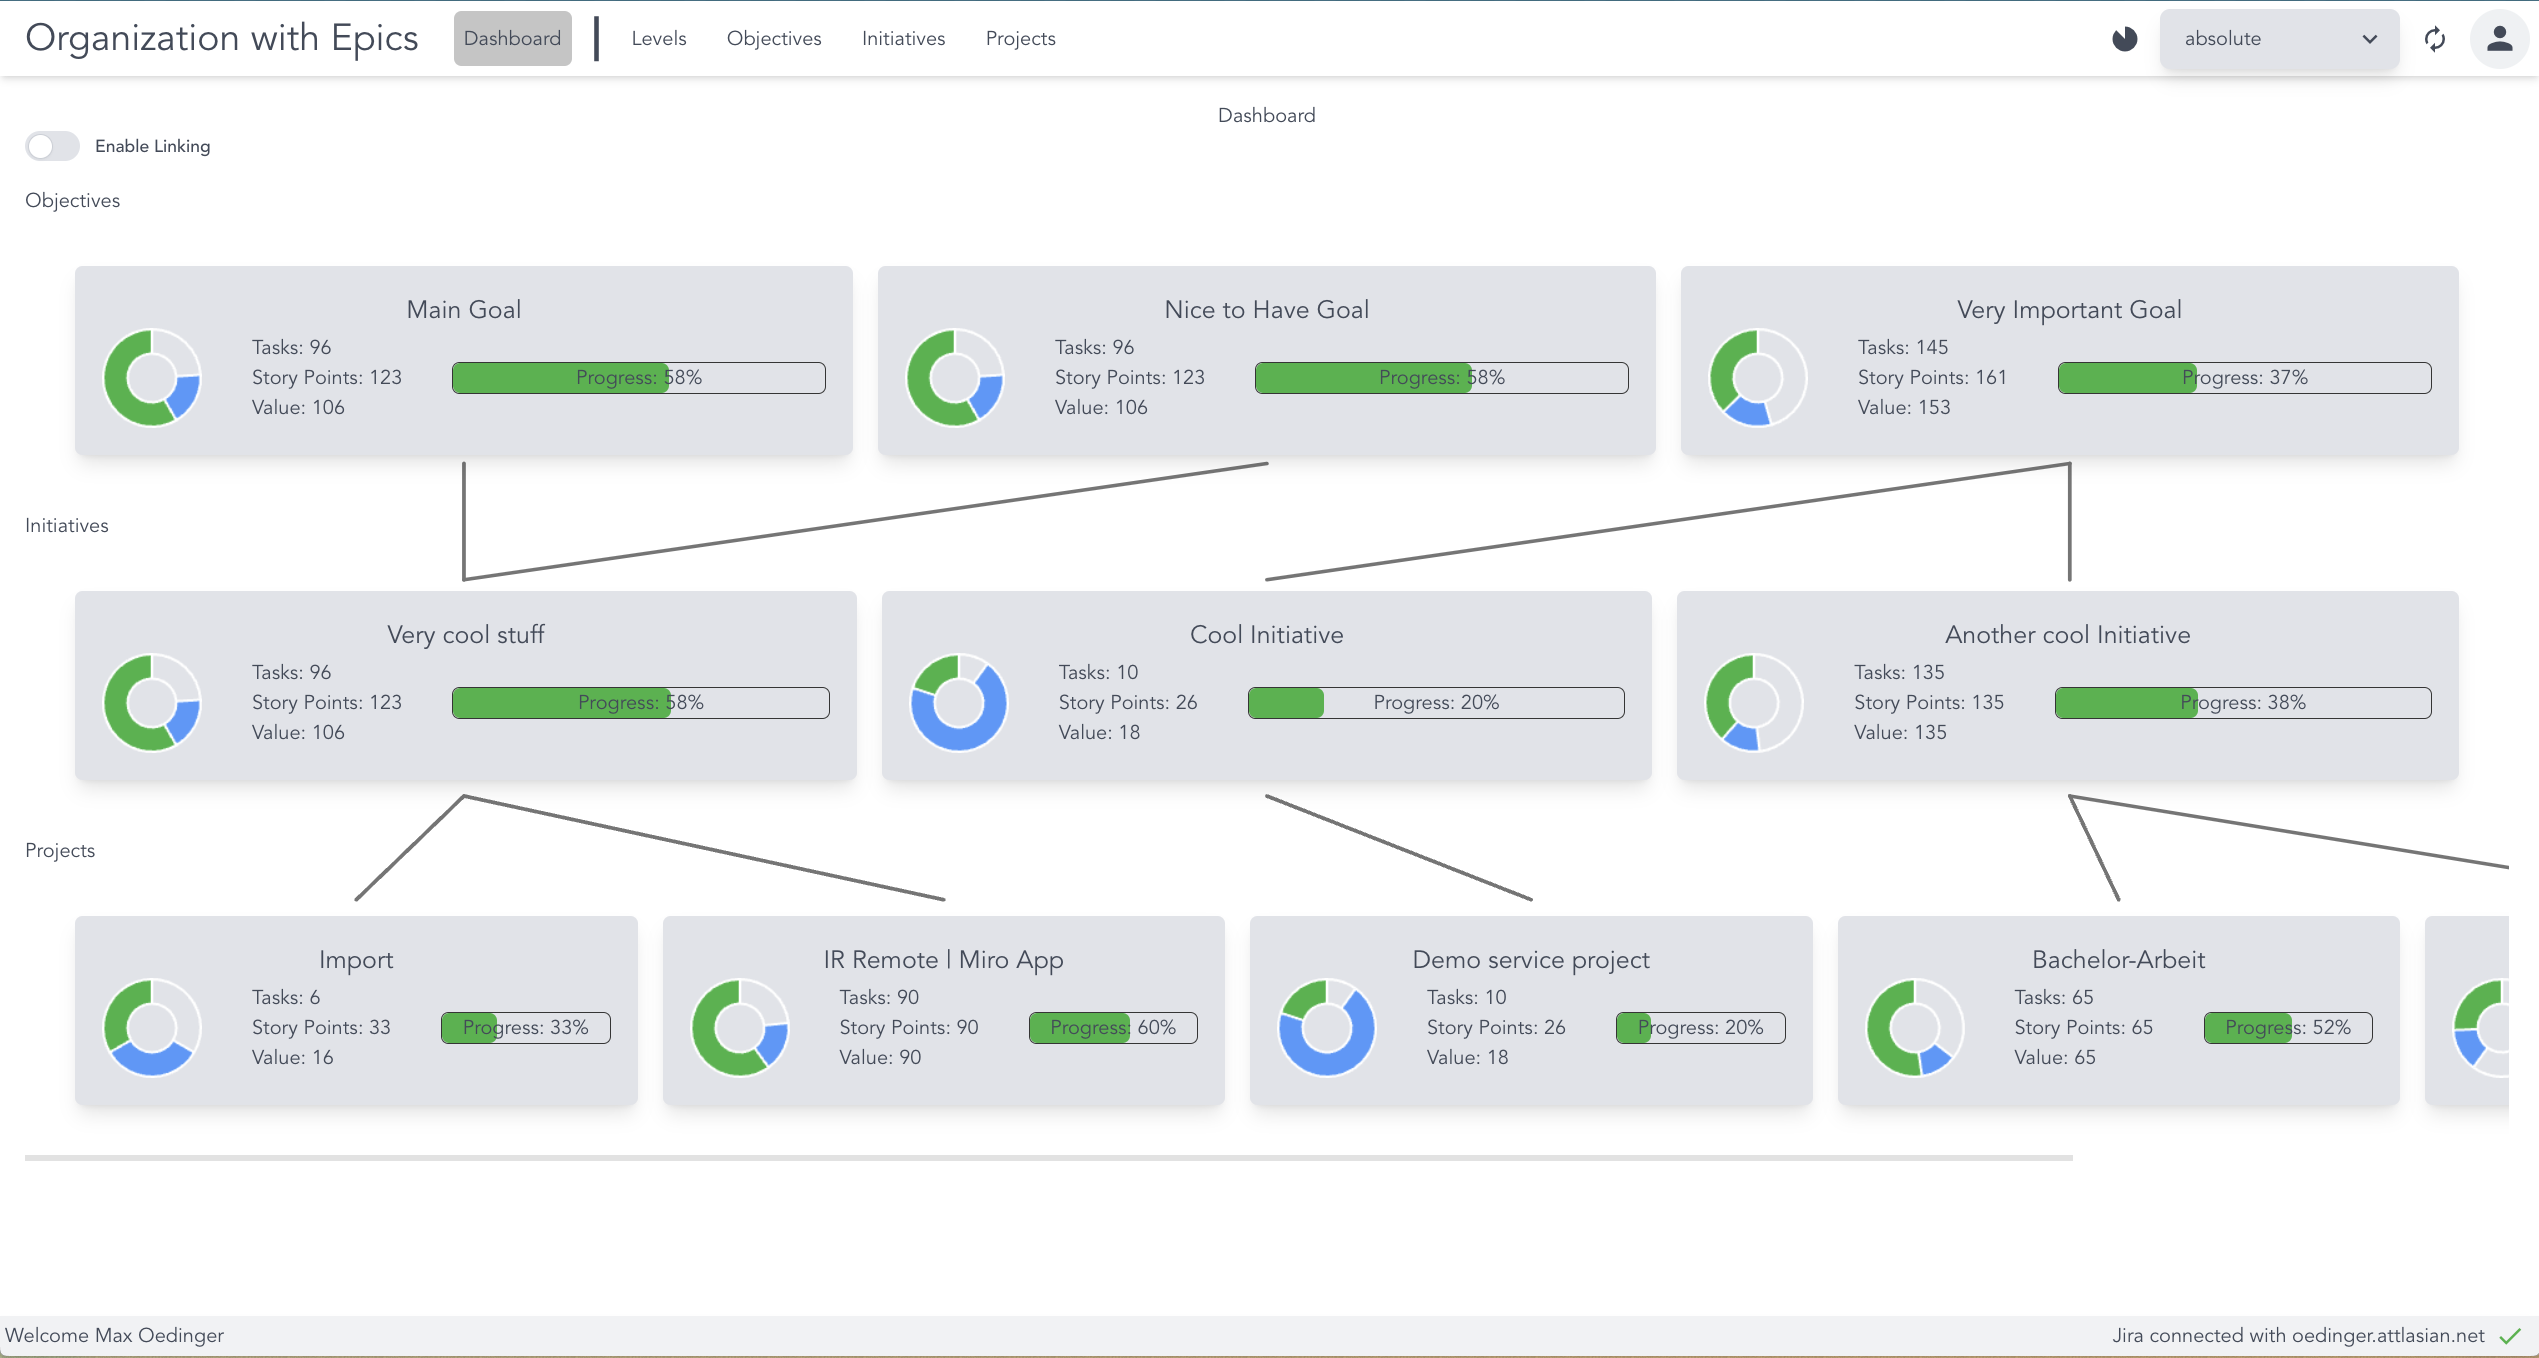
\includegraphics[width=\linewidth]{Dashboard_withScroll}
        \captionof{figure}{Dashboard mit scrollbaren Gruppen}
    \end{minipage}
\end{center}
\vspace{20pt}

Der Nutzer hat die Möglichkeit Verlinkung über ein Toggle zu aktivieren, wodurch über jeder Gruppe, die verlinkt werden kann, ein Punkt erscheint, den der Nutzer mit Drag-and-Drop verwenden kann, um die Gruppe mit einer anderen Gruppe zu verbinden.
Anhand der Start-Position und aktuellen Position des Mauszeigers wird währenddessen eine neue Linie dargestellt, die dem Nutzer zeigt, wie die Verbindung aussieht, die er erzeugt. Anschließend werden die Verbindungslinien anhand der neuen Positionen der Gruppen erneut berechnet.

Zusätzlich zu den Linien kann der Nutzer den Mauszeiger über eine Gruppe bewegen, wodurch die Gruppe und die Gruppen, die mit dieser Gruppe verknüpft sind, inklusive aller relevanten Verbindungslinien, blau hervorgehoben werden.

\vspace{20pt}
\begin{center}
    \begin{minipage}{1\linewidth}
        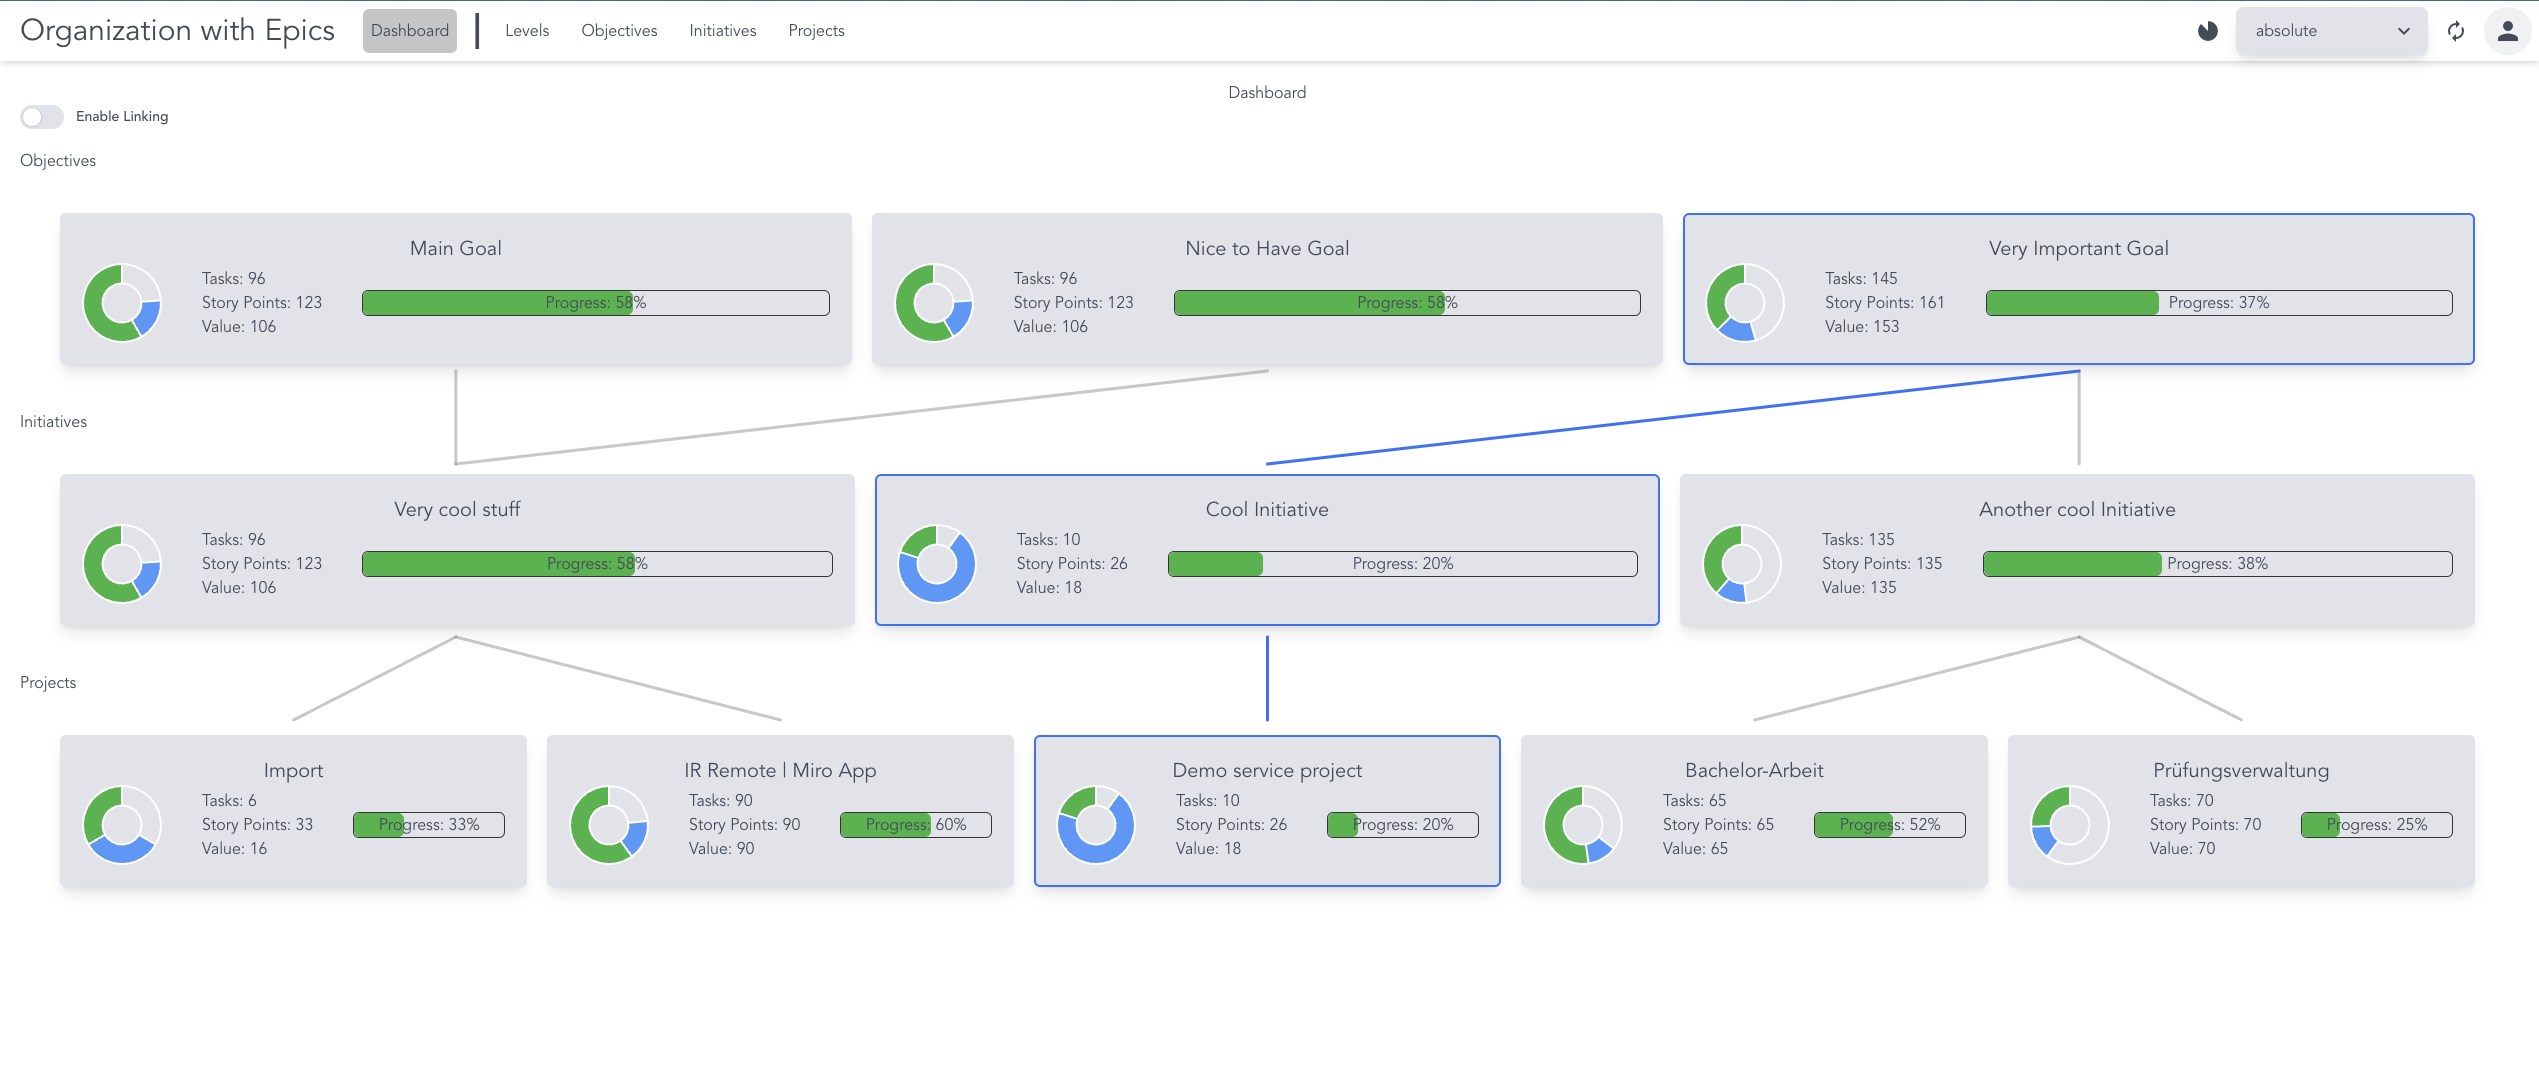
\includegraphics[width=\linewidth]{Dashboard_withHighlighting}
        \captionof{figure}{Dashboard mit hervorgehobenen Gruppen}
    \end{minipage}
\end{center}
\vspace{20pt}

Für die Erzeugung der Doughnut-Diagramme wird Chart.js verwendet, da es eine simple und visuell ansprechende Möglichkeit bietet einfache Diagramme zu erstellen. Durch das Plugin Vue-Chartjs gibt es die Möglichkeit die Diagramme in Vue.js direkt als Komponente einzubinden, was die Verwendung weiter erleichtert.

\subsection{lokale Inbetriebnahme}
Um die Anwendung zu starten werden zwei Möglichkeiten angeboten. Die erste Möglichkeit besteht in der Verwendung von Docker-Compose. Die zweite Möglichkeit besteht in der Verwendung von Node.js, Vite, und Docker für die MongoDB.
Detailierte Beschreibungen für die konkreten Details der Inbetriebnahme sind in der \verb|README.md|-Datei im \verb|prototype|-Ordner des \href{https://github.com/Max-0e/bachelor/blob/main/prototype/README.md}{Repositories} zu finden.

\subsection{CI/CD}
Für eine schnelle und einfache Möglichkeit die Anwendung als produktive Anwendung zu testen und Verbesserungen zu deployen wurde eine CI/CD-Pipeline mit GitHub-Actions eingerichtet. Die GitHub-Action definiert, wann die Pipeline ausgeführt werden soll und welche Schritte in der Pipeline ausgeführt werden sollen. Der Trigger für die Pipeline ist hier das Mergen und daraus resultierenden Schließen eines Pullrequests der als Ziel den main-Branch des Repositories hat.

\begin{lstlisting}[caption=GitHub-Action]
name: Docker Image CI/CD Pipeline

on:
    pull_request:
    types:
        - closed
    branches:
        - main

jobs:
    build:
    if: github.event.pull_request.merged == true
    runs-on: self-hosted 
    environment: 
        name: production
    env:
        MONGO_PASSWORD: ${{ secrets.MONGO_PASSWORD }}
        SECRET: ${{ secrets.SECRET }}
        CLIENT_APP_URL: ${{ vars.CLIENT_APP_URL }}
        MONGO_DB: ${{ vars.MONGO_DB }}
        MONGO_URL: ${{ vars.MONGO_URL }}
        MONGO_USER: ${{ vars.MONGO_USER }}
        SMTP_HOST: ${{ vars.SMTP_HOST }}
        SMTP_PORT: ${{ vars.SMTP_PORT }}
        SMTP_USER: ${{ vars.SMTP_USER }}
        VITE_API_URL: ${{ vars.VITE_API_URL }}
        VITE_APP_DEV_MODE: ${{ vars.VITE_APP_DEV_MODE }}
    steps:
    - uses: actions/checkout@v3
    - name: Build the Docker image
        run: 
        cd prototype && 
        docker build . --file "Dockerfile" --tag bachelor:latest 
        --build-arg MONGO_PASSWORD=${{ env.MONGO_PASSWORD }}
        --build-arg SECRET=${{ env.SECRET }}
        --build-arg CLIENT_APP_URL=${{ env.CLIENT_APP_URL }}
        --build-arg MONGO_DB=${{ env.MONGO_DB }}
        --build-arg MONGO_URL=${{ env.MONGO_URL }}
        --build-arg MONGO_USER=${{ env.MONGO_USER }}
        --build-arg SMTP_HOST=${{ env.SMTP_HOST }}
        --build-arg SMTP_PORT=${{ env.SMTP_PORT }}
        --build-arg SMTP_USER=${{ env.SMTP_USER }}
        --build-arg SMTP_PASS=${{ env.SMTP_PASS }}
        --build-arg VITE_API_URL=${{ env.VITE_API_URL }}
        --build-arg VITE_DEV_MODE=${{ env.VITE_APP_DEV_MODE }}
    deploy:
    needs: build
    runs-on: self-hosted
    environment: 
        name: production
    env:
        MONGO_PASSWORD: ${{ secrets.MONGO_PASSWORD }}
        SECRET: ${{ secrets.SECRET }}
        CLIENT_APP_URL: ${{ vars.CLIENT_APP_URL }}
        MONGO_DB: ${{ vars.MONGO_DB }}
        MONGO_URL: ${{ vars.MONGO_URL }}
        MONGO_USER: ${{ vars.MONGO_USER }}
        SMTP_HOST: ${{ vars.SMTP_HOST }}
        SMTP_PORT: ${{ vars.SMTP_PORT }}
        SMTP_USER: ${{ vars.SMTP_USER }}
        SMTP_PASS: ${{ secrets.SMTP_PASS }}
    steps:
        - name: Deploy the newest Docker image
        run: docker compose -f "prototype/docker-compose.ci.yml" up -d
        - name: Delete all old and unused Images
        run: docker system prune -af
\end{lstlisting}

Die Pipeline besteht aus zwei Teilen, sogenannten Jobs: Build und Deploy.
Build erzeugt aus dem geupdateten Quellcode ein neues Docker-Image nach den konkreten Anweisungen die in dem Dockerfile im root-Verzeichnis des Prototypen definiert sind. Bei dem Dockerfile handelt es sich um ein multi-stage Dockerfile, welches in drei Schritten ein Image erzeugt. Diese drei Schritte sind:
frontend-build, backend-build, und production.

\begin{lstlisting}[caption=Dockerfile zum Bauen des Images]
# build stage
# frontend
FROM node:16-alpine as fe-build-stage
WORKDIR /app
ARG VITE_API_URL
ARG VITE_DEV_MODE
COPY ./frontend/package*.json .
RUN npm ci
COPY ./frontend/ .
RUN npm run build:ci

# backend
FROM node:16-alpine as be-build-stage
WORKDIR /app
COPY ./backend/package*.json .
RUN npm ci
COPY ./backend .
RUN npm run build
RUN mkdir ./build/views
RUN mkdir ./build/views/frontend
COPY --from=fe-build-stage /app/dist ./build/views/frontend


# production stage
FROM node:16-alpine as production-stage
WORKDIR /app
COPY ./backend/package*.json ./
RUN npm ci
COPY --from=be-build-stage /app/build /app
EXPOSE 3000
CMD [ "node", "./main.js"]
\end{lstlisting}

Im ersten Schritt wird der Frontend-Code kompiliert. Im zweiten Schritt wird der Backend-Code kompiliert und das kompilierte Frontend aus dem ersten Schritt zur statischen Auslieferung in einen bestimmten Ordner kopiert. Im dritten Schritt wird ein Node-Image für die Produktivumgebung erzeugt, welches das kompilierte Backend inklusive des Frontends enthält und mit einem Start-Befehl der Webserver gestartet wird.
Das resultierende Image, welches nun eine lauffähige Version der Anwendung enthält, wird anschließend als neueste Version des Images getagt.
Deploy führt ein Update der konkreten Produktivumgebung durch. Dazu wird das Image, welches im Build-Job erzeugt wurde, und das laufende Image ersetzt. Hierzu wird die Docker-Compose-Datei verwendet, welche die Konfiguration der Docker-Services der Produktivumgebung beschreibt. Diese Datei referenziert immer die neueste Version des gebauten Images und einen Reverse-Proxy-Service von "Traefik", welcher dazu dient das Portmapping auf dem Server zu übernehmen und mithilfe von Letsencrypt ein SSL-Zertifikat für die angegebene Domain auszustellen.
Zuletzt werden alle alten und unbenutzten Images gelöscht.

Die Datenbank für den Produktiv-Server ist eine konstenlose Version einer Cloud-Instanz von Mongo-Atlas.